%! Author = Deniz Altunkapan

% Preamble
\documentclass{article}

% Packages
% \usepackage[options]{packagename}
\usepackage[utf8]{inputenc}
\usepackage[T1]{fontenc}
\usepackage[ngerman]{babel}
\usepackage{lmodern}
\usepackage{graphicx}
\usepackage[pdftex,hyperref,dvipsnames]{xcolor}
\usepackage{listings}
\usepackage[a4paper,lmargin={2cm},rmargin={2cm},tmargin={3.5cm},bmargin = {2.5cm},headheight = {4cm}]{geometry}
\usepackage{amsmath,amssymb,amstext,amsthm}
% \usepackage[lined,algonl,boxed]{algorithm2e}
% alternative zu algorithm2e:
%\usepackage[]{algorithm} %counter mit chapter
%\usepackage{algpseudocode}
\usepackage{tikz-qtree}
\usepackage{tikz}
\usepackage{hyperref}
\usepackage{url}
\usepackage[inline]{enumitem} % Ermöglicht ändern der enum Item Zahlen
\usepackage[headsepline]{scrlayer-scrpage} 
\pagestyle{scrheadings} 
\usetikzlibrary{automata,positioning}
\usepackage{forest}

% Format and Header
% Überschreibt enumerate Befehl, sodass 1. Ebene Items mit
\renewcommand{\theenumi}{(\alph{enumi})}
% (a), (b), etc. nummeriert werden.
\renewcommand{\labelenumi}{\text{\theenumi}}

% Counter für das Blatt und die Aufgabennummer.
% Ersetze die Nummer des Übungsblattes und die Nummer der Aufgabe
% den Anforderungen entsprechend.
% Gesetzt werden die counter in der hauptdatei, damit sie hier nicht jedes mal verändert werden muss
% Beachte:
% \setcounter{countername}{number}: Legt den Wert des Counters fest
% \stepcounter{countername}: Erhöht den Wert des Counters um 1.
\newcounter{sheetnr}
\newcounter{exnum}

% Befehl für die Aufgabentitel
\newcommand{\exercise}[1]{\section*{Aufgabe \theexnum\stepcounter{exnum}: #1}} % Befehl für Aufgabentitel

% Formatierung der Kopfzeile
% \ohead: Setzt rechten Teil der Kopfzeile mit
% Namen und Matrikelnummern aller Bearbeiter
\ohead{Deniz Altunkapan| 3721629| st187784}
\ofoot[\pagemark]{\pagemark}
% \chead{} kann mittleren Kopfzeilen Teil sezten
% \ihead: Setzt linken Teil der Kopfzeile mit
% Modulnamen, Semester und Übungsblattnummer
\ihead{Zusammenfassung Einführung Software Engineering 2024 SS
%Blatt \thesheetnr
}

% Sheet and exercise counter
\setcounter{sheetnr}{1}
\setcounter{exnum}{1}

% Own packages
\usepackage{pdfpages}
\usepackage{tikz-qtree}

% Own declaration

% This is used to format the jave-code-block
% copied from StackOverflow
\definecolor{dkgreen}{rgb}{0,0.6,0}
\definecolor{gray}{rgb}{0.5,0.5,0.5}
\definecolor{mauve}{rgb}{0.58,0,0.82}
\lstset{frame=tb,
  language=Java,
  aboveskip=3mm,
  belowskip=3mm,
  showstringspaces=false,
  columns=flexible,
  basicstyle=\small,
  keywordstyle=\bfseries,
  numbers=left,
  numberstyle=\tiny\color{black},
  commentstyle=\color{dkgreen},
  stringstyle=\color{mauve},
  breaklines=true,
  breakatwhitespace=true,
  tabsize=3,
  frame=single
}

% this is used used for pseudocode
\lstnewenvironment{algorithm}[1][] %defines the algorithm listing environment
{   
    \lstset{ %this is the stype
        mathescape=true,
        frame=tB,
        numbers=left, 
        numberstyle=\tiny,
        basicstyle=\scriptsize, 
        keywordstyle=\color{black}\bfseries\em,
        keywords={,input, output, return, datatype, function, in, if, else, foreach, while, begin, end, do, od, fi, } %add the keywords you want, or load a language as Rubens explains in his comment above.
        numbers=left,
        xleftmargin=.04\textwidth,
        #1 % this is to add specific settings to an usage of this environment (for instnce, the caption and referable label)
    }
}
{}

% Document
\begin{document}
\tableofcontents
\newpage
\section*{Anforderungsanalyse}
\addcontentsline{toc}{section}{Anforderungsanalyse}
  \begin{enumerate}[label=\alph*)]
   \item
\addcontentsline{toc}{subsection}{Use Case Diagram/ Use Case Table}
   \underline{Use Case Diagram/ Use Case Table}\\
   
   Mit dem Use Case Diagramm werden von außen sichtbare Interaktionen von Akteuren visualisiert. Damit beschreibt es in einer hohen Abstraktion, welche Funktionen und Dienste ein System für einen Anwender bereitstellt.\\ Ein Use Case Table (Anwendungsfalltabelle) ist ein Werkzeug, das in der Softwareentwicklung und im Projektmanagement verwendet wird, um verschiedene Anwendungsfälle eines Systems zu dokumentieren. Diese Tabelle hilft dabei, die Anforderungen und Interaktionen zwischen den Benutzern (Akteuren) und dem System zu verstehen und zu spezifizieren.\\
  	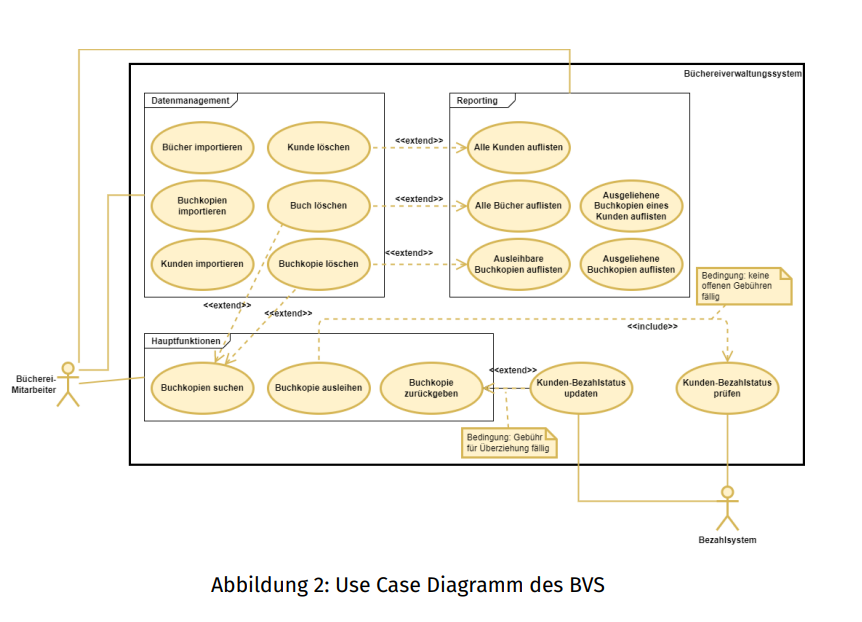
\includegraphics[scale=1.1]{media/useCase.png}
  	
  	Die «include»-Beziehung zeigt an, dass ein Anwendungsfall den Ablauf eines anderen Anwendungsfalls einschließt. Das bedeutet, dass der inkludierte Anwendungsfall immer dann ausgeführt wird, wenn der Hauptanwendungsfall ausgeführt wird.\\
  	Syntax: Ein gestrichelter Pfeil mit einem offenen Pfeilkopf, der von dem Hauptanwendungsfall zum inkludierten Anwendungsfall zeigt, mit der Beschriftung «include».\\
  	
  	Die «extend»-Beziehung zeigt an, dass ein Anwendungsfall den Ablauf eines anderen Anwendungsfalls erweitert. Dies bedeutet, dass der erweiternde Anwendungsfall optional ist und nur unter bestimmten Bedingungen ausgeführt wird.\\
  	Syntax: Ein gestrichelter Pfeil mit einem offenen Pfeilkopf, der von dem erweiternden Anwendungsfall zum erweiterten Anwendungsfall zeigt, mit der Beschriftung «extend».\\
  		
\newpage

  	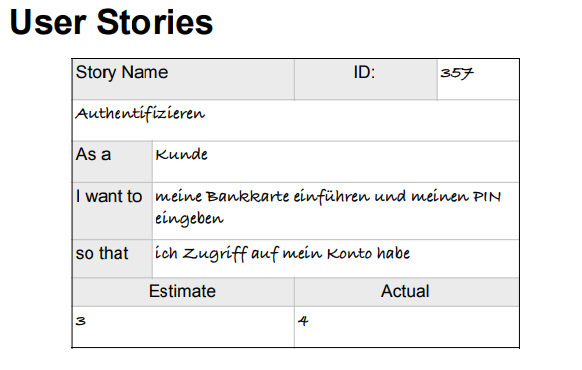
\includegraphics[scale=1]{media/userStories}\\
  	Hierbei bezeichnet 'Estimate' die Aufwandsabschätzung.
  	
  	\includegraphics[scale=1.2]{media/useCaseTable4}	
\subsection*{Ist- und Soll-Analyse}
\addcontentsline{toc}{subsection}{Ist- und Soll-Analyse}
Eine Soll-Ist-Analyse in der Softwareentwicklung ist eine Methode zur Identifikation und Analyse von Unterschieden zwischen dem aktuellen Zustand eines Systems oder Prozesses (Ist-Zustand,bspw. Auswertung vorhandener Daten, Dokumente) und dem gewünschten oder geplanten Zustand (Soll-Zustand,bspw. Prototyping). Diese Analyse wird oft eingesetzt, um Verbesserungsmöglichkeiten zu identifizieren, Abweichungen zu verstehen und entsprechende Maßnahmen zur Anpassung oder Optimierung zu entwickeln.
\newpage

\addcontentsline{toc}{subsection}{INVEST- Kriterien (Qualitätskriterien einer User Story)}
   \item \subsection*{INVEST- Kriterien (Qualitätskriterien einer User Story)} 
   \textbf{I}ndependent: Jede User Story sollte unabhängig von anderen sein\\
   \textbf{N}egotiable: Storys müssen verhandelbar sein und Details müssen während der Entwicklung anpassbar sein\\
   \textbf{V}aluable: stellt sicher, dass jede Story einen Wert für den Kunden hat, sollte Mehrwert für Nutzer und Produkt darstellen (auch zukünftig)\\
   \textbf{E}stimable: Man sollte in der Lage sein die Arbeit abzuschätzen (sonst split/slicing)\\
   \textbf{S}ized Appropriately (Small): Story sollte so klein wie möglich sein\\
   \textbf{T}estable: Story sollte testbar sein (Akzeptanzkriterien)\\
   
   
\includegraphics[scale=1.18]{media/Invest.png}
   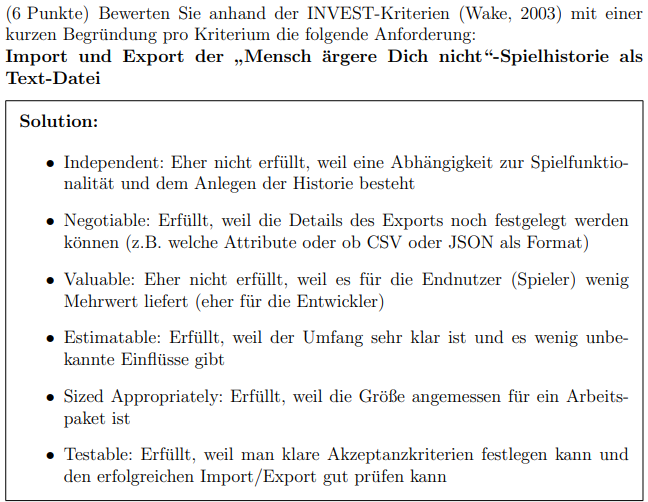
\includegraphics[scale=0.88]{media/Invest2.png}

\newpage

\addcontentsline{toc}{subsection}{Funktionale und Nichtfunktionale Anforderungen}   
   \item \subsection*{Funktionale und Nichtfunktionale Anforderungen}
   \textbf{Funktionale Anforderungen}(Problemorientiert, Abstrakt) beschreiben die spezifischen Funktionen und Verhaltensweisen, die ein System ausführen soll. Sie definieren, was das System tun soll und wie es auf bestimmte Eingaben reagieren soll. Funktionale Anforderungen beziehen sich auf konkrete Features, Aufgaben oder Interaktionen des Systems mit Benutzern oder anderen Systemen.\\
   \textbf{Nichtfunktionale Anforderungen}(Konkret, Präzise) beschreiben die Qualitätseigenschaften und die allgemeinen Bedingungen, unter denen das System arbeitet. Sie definieren, wie das System seine Funktionen ausführen soll und beziehen sich oft auf Leistungsmerkmale, Sicherheitsanforderungen, Wartbarkeit, Skalierbarkeit und Benutzerfreundlichkeit.
   
   \underline{Beispiele des BVS:}\\ Funktionale Anforderungen:\\
1. Importieren einer CSV-Datei mit Büchern:
• via absoluten oder relativen Pfad zu einem CSV-File
• Inhalt wird gelesen und ins System eingespeist (eine Zeile entspricht einer Buchkopie)
• Struktur: isbn;title;authors;year;city;publisher;edition\\
 Nicht-Funktionale Anforderungen:\\
Wichtige nicht-funktionale Anforderungen sind zum einen die Verwendung der Programmiersprache Java und die Kompatibilität mit Java 17 SE.
Weiterhin sind Effizienz und Benutzerfreundlichkeit der Kommandozeilensteuerung
sehr wichtig. Die Menüanordnung und -auswahl sollen auf die wichtigsten Prozesse
(8, 9, 7) ausgerichtet sein, sodass diese möglichst schnell erreichbar sind.

\addcontentsline{toc}{subsection}{Lastenheft und Pflichtenheft}	
   \item \subsection*{Lastenheft und Pflichtenheft}
   Das Lastenheft ist ein Dokument, das vom Auftraggeber erstellt wird und beschreibt, was das System leisten soll. Es enthält die Anforderungen und Wünsche des Auftraggebers an das System.\\
   Das Pflichtenheft ist ein Dokument, das vom Auftragnehmer erstellt wird und beschreibt, wie die im Lastenheft definierten Anforderungen technisch umgesetzt werden sollen.\\
   
   \underline{Zweck:}\\
\textbf{Lastenheft:} Beschreibt die Anforderungen und Wünsche des Auftraggebers an das System (Was soll das System leisten?).\\
\textbf{Pflichtenheft:} Beschreibt die technische Umsetzung der Anforderungen des Auftraggebers (Wie sollen die Anforderungen umgesetzt werden?).\\

   \underline{Inhaltliche Tiefe:}\\
\textbf{Lastenheft:} Enthält allgemeine Anforderungen und Rahmenbedingungen.\\
\textbf{Pflichtenheft:} Enthält detaillierte technische Spezifikationen und Implementierungspläne.


\item \subsection*{Verifikation und Validierung}
\addcontentsline{toc}{subsection}{Verifiktion und Validierung}
\textbf{Verifikation} bezieht sich auf den Prozess der Überprüfung, ob die Software gemäß den Spezifikationen und Entwürfen korrekt implementiert wurde. Es geht darum, sicherzustellen, dass das Produkt "richtig gebaut" wurde. Verifikation wird oft durch verschiedene technische Aktivitäten wie Code-Inspektionen, Reviews, statische Analysen und Unit-Tests durchgeführt.\\

Frage: Bauen wir das Produkt richtig?\\

\textbf{Validierung} bezieht sich auf den Prozess der Überprüfung, ob die Software die tatsächlichen Bedürfnisse und Erwartungen der Benutzer erfüllt. Es geht darum, sicherzustellen, dass das Produkt "das richtige Produkt" ist. Validierung wird oft durch Aktivitäten wie Systemtests, Akzeptanztests und Benutzerfeedback durchgeführt.\\

Frage: Bauen wir das richtige Produkt?\\

\end{enumerate}
\newpage
\addcontentsline{toc}{section}{Entwurf}
\section*{Entwurf}
  \begin{enumerate}[label=\alph*)]
\addcontentsline{toc}{subsection}{Komponentendiagram}
   \item \underline{Komponentendiagram}\\
   
   Eine \textbf{Komponente} ist ein ersetzbarer und modularer Bestandteil eines Systems. Eine Komponente ist eine Einheit, die eine bestimmte Funktionalität kapselt und in einem größeren System eingebaut werden kann. Sie kann aus einer Sammlung von Klassen bestehen, muss es aber nicht.\\
   Eine \textbf{Schnittstelle} ist eine Methode oder ein Satz von Methoden, die von einer anderen Komponente verwendet werden. Eine bestimmte Komponente kann anderen Komponenten Schnittstellen zur Verfügung stellen und/oder Schnittstellen von anderen Komponenten benötigen.
   
 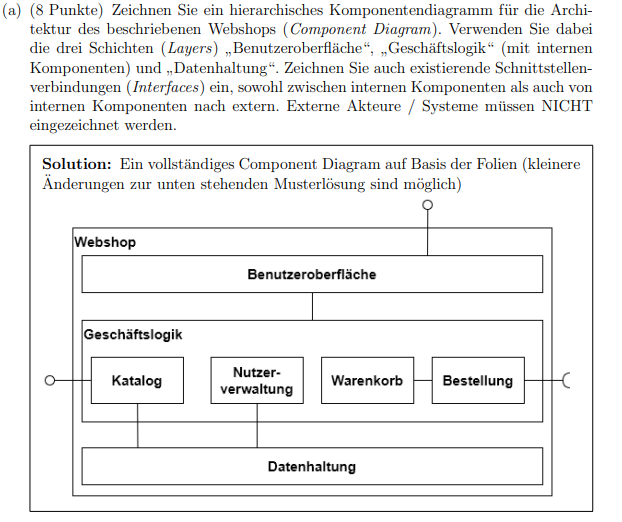
\includegraphics[scale=1]{media/componentDiagram.png}
   
\item \subsection*{Grobentwurf vs. Feinentwurf}
\addcontentsline{toc}{subsection}{Grobentwurf vs. Feinentwurf}
\textbf{Detailtiefe:}\\
Grobentwurf: Behandelt die Systemarchitektur und die Hauptkomponenten auf einer hohen Abstraktionsebene. Er legt die Struktur und die wesentlichen Interaktionen fest, ohne in die Details der Implementierung zu gehen.\\
Feinentwurf: Behandelt die Details der einzelnen Komponenten und deren Implementierung. Er liefert konkrete Anweisungen für die Programmierung und beschreibt die spezifischen Designaspekte.\\
\textbf{Zielsetzung:}\\
Grobentwurf: Ziel ist es, eine klare, strukturierte Übersicht über das System zu bieten und die grundlegenden Designentscheidungen zu treffen.\\
Feinentwurf: Ziel ist es, die genaue technische Umsetzung der Komponenten zu planen und die Implementierung vorzubereiten.\\
\textbf{Ergebnisse:}\\
Grobentwurf: Architekturdiagramme und grundlegende Designentscheidungen.\\
Feinentwurf: Detaillierte Diagramme, Spezifikationen und Anweisungen für die Implementierung.\\

\addcontentsline{toc}{subsection}{Entwurfs- und Architekturmuster (Patterns)} 
   \item \subsection*{Entwurfs- und Architekturmuster (Patterns)}
   \subsubsection*{Singleton Pattern}
   \addcontentsline{toc}{subsubsection}{Singleton Pattern}
   • Es soll sichergestellt werden, dass es zu einer Klasse höchstens eine Instanz gibt\\
   • Diese Instanz soll global verfügbar sein, d.h. es muss eine Möglichkeit für alle Objekte geben, diese Instanz anzusprechen.
   \begin{lstlisting}
public class Singleton {
    private static Singleton instance;
    private Singleton() { // privater Konstruktor verhindert Instanzierung}
    
    public static synchronized Singleton getInstance() {
        if (instance == null) {instance = new Singleton();}
        return instance;
    }
}
   \end{lstlisting}
  
\addcontentsline{toc}{subsubsection}{Composite Pattern}
   \subsubsection*{Composite Pattern}
   • Designmuster , mit dem man Objekte in baumartige Strukturen zusammensetzen kann, um Teil-Ganzes-Hierarchien darzustellen. Es ermöglicht Clients, einzelne Objekte und Objektkompositionen einheitlich zu behandeln. Mit anderen Worten: Unabhängig davon, ob es sich um ein einzelnes Objekt oder eine Gruppe von Objekten (Composite) handelt, können Clients sie austauschbar verwenden.\\
   • Es wird verwendet, um Baumstrukturen darzustellen und die Arbeit mit Einzelobjekten und zusammengesetzten Objekten einheitlich zu gestalten.\\
   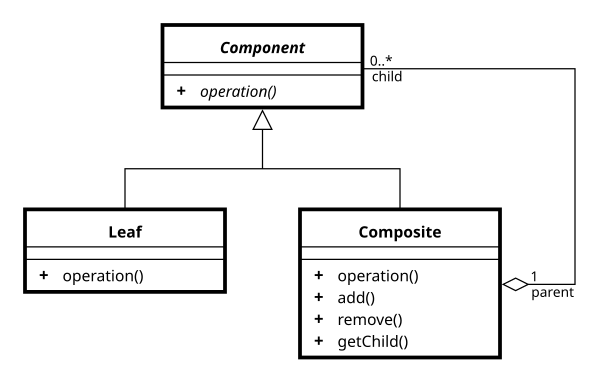
\includegraphics[scale=0.4]{media/compositePattern.png}
   
   
\addcontentsline{toc}{subsubsection}{State Pattern}
   \subsubsection*{State Pattern}
   • Ein Objekt soll sich abghängig von seinem Zustand verschieden verhalten.\\
   • Der Zustand wird als Klasse gekapselt. Spezielle Zustandsklassen mit überladenen Methoden implementieren die jeweilige Zustandsabhängigkeit.\\
   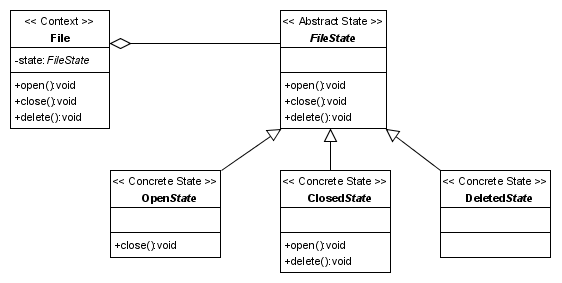
\includegraphics[scale=0.45]{media/statePattern.png}
   
\addcontentsline{toc}{subsubsection}{Drei-Schichten-Architektur}
   \subsubsection*{Drei-Schichten-Architektur}
   Sie teilt die Anwendung in drei logische Schichten auf, um die Komplexität zu reduzieren und die Wartbarkeit zu verbessern. Diese Schichten sind:\\
   • Präsentationsschicht (client tier, Front-End): Ist für die Präsentation und die Eingabe der Daten \\(die Benutzerschnittstelle) verantwortlich.\\
   • Logikschicht (application-server tier): Verarbeitung der Daten.Hier ist die Anwendungslogik vereint.\\
   • Datenhaltungssschicht (data-server tier, back end): Sie enthält die Datenbank und ist verantwortlich für das Speichern und Laden von Daten.\\
	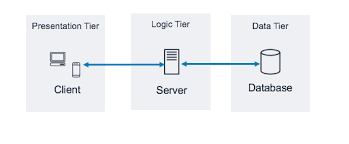
\includegraphics[scale=0.6]{media/3LayerArch.png}
	
\addcontentsline{toc}{subsubsection}{Pipe-Filter-Architektur}
   \subsubsection*{Pipe-Filter-Architektur}
   Das Pipe-Filter-Architekturmuster dient dazu, eine Anwendung zu strukturieren, die Daten auf einem
virtuellen Fließband verarbeitet.\\
   • Die Verarbeitungsschritte werden in den sogenannten Filtern realisiert. Ein Filter verbraucht und erzeugt
Daten.\\
   • Pipes leiten die Ergebnisse des Filters an nachfolgende Filter weiter.\\
   • Das erste Filter bekommt seine Daten aus der Datenquelle, das letzte liefert sie an die Datensenke. \\
   
   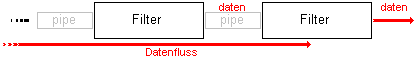
\includegraphics[scale=0.6]{media/PipesFilters.png}
   
   
\addcontentsline{toc}{subsubsection}{Microservices-Architektur}
   \subsubsection*{Microservices-Architektur}
   Die Mikroservices-Architektur ist ein Ansatz in der Softwareentwicklung, bei dem eine Anwendung als eine Sammlung von kleinen, unabhängigen Diensten oder Mikroservices entwickelt wird. Jeder dieser Dienste ist für eine spezifische Geschäftsaufgabe verantwortlich und kann unabhängig voneinander entwickelt, bereitgestellt und skaliert werden. Diese Architektur hat sich als Alternative zur monolithischen Architektur etabliert, insbesondere bei komplexen und großen Systemen.
   
   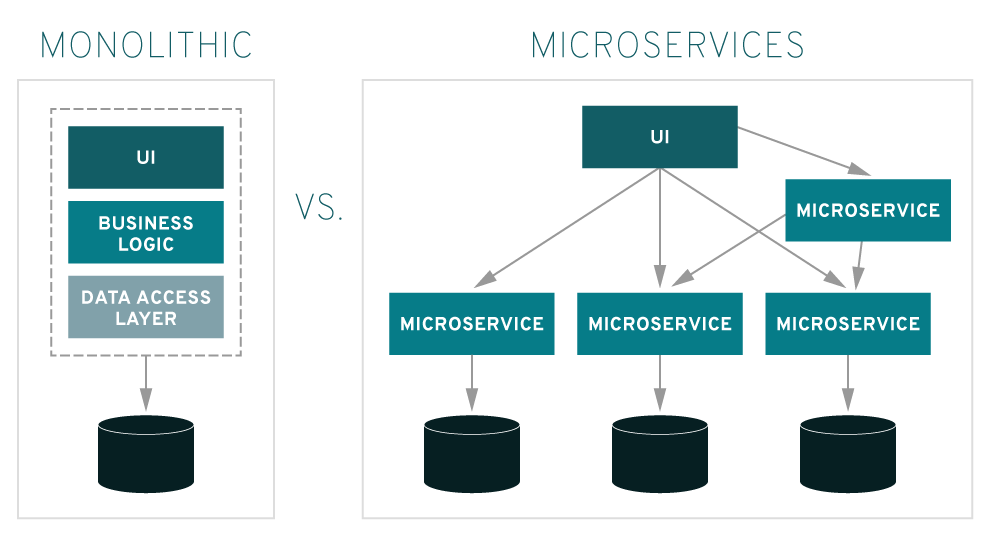
\includegraphics[scale=0.3]{media/microArch.png}

\newpage 
\addcontentsline{toc}{subsection}{Domain Driven Design}
   \item \subsection*{Domain Driven Design}
   Domain-Driven Design (DDD) ist ein Ansatz zur Softwareentwicklung, der den Fokus auf die Modellierung der Domäne (das spezifische Fachgebiet, für das die Software entwickelt wird) legt. DDD wurde von Eric Evans in seinem Buch Domain-Driven Design: Tackling Complexity in the Heart of Software eingeführt.
Die Geschäftslogik, Anforderungen und der Bereich, den das System adressiert stehen im Mittelpunkt der Softwareentwicklung. Entwickler und Fachexperten arbeiten eng zusammen, um ein tiefes Verständnis der Domäne zu entwickeln.\\
\textbf{Kernkonzepte:}
\begin{enumerate}[label=\arabic*)]
\item Ubiquitous Language (Allgegenwärtige Sprache)

Eine gemeinsame Sprache, die von allen Beteiligten (Entwicklern und Fachexperten) verwendet wird. Diese Sprache umfasst alle relevanten Begriffe und Konzepte der Domäne und wird in allen Kommunikationsformen und im Code konsequent verwendet.
\item Bounded Context (Begrenzter Kontext)

Ein Bounded Context definiert klare Grenzen für ein bestimmtes Domänenmodell und die zugehörige Ubiquitous Language. Innerhalb eines Bounded Contexts sind die Begriffe und Regeln einheitlich und klar definiert. Dies hilft, die Komplexität großer Systeme durch klare Abgrenzungen zu reduzieren und Missverständnisse zu vermeiden. 
\item Entity

Eine Entity ist ein Objekt, das durch seine Identität definiert ist. Es hat eine eigenständige Lebensdauer und kann sich im Laufe der Zeit ändern, behält aber seine Identität bei. Beispiele sind Kunden, Bestellungen oder Produkte.
\item Value Objects

Objekte, die durch ihre Eigenschaften definiert sind und keine eigene Identität besitzen. Beispielsweise könnte eine Adresse ein Value Object sein, da sie nur durch die Kombination ihrer Felder (Straße, Stadt, Postleitzahl) definiert ist.
\item Aggregate

Ein Aggregate ist eine Gruppe von zusammengehörigen Objekten (Entities und Value Objects), die als Einheit behandelt werden. Es hat eine Wurzel-Entity (Aggregate Root), die die Konsistenz und Integrität des gesamten Aggregates gewährleistet.
\item Repository

Ein Repository ist eine Abstraktion für die Speicherung und das Abrufen von Aggregates. Es bietet eine Sammlung ähnlicher Objekte und kapselt die Implementierung der Datenzugriffslogik.
\item Service

Ein Service ist eine Operation oder eine Gruppe von Operationen, die nicht natürlich zu einer Entity oder einem Value Object gehören. Services sind oft zustandslos und bieten domänenspezifische Funktionalitäten.
\item Domain Event

Ein Domain Event signalisiert, dass innerhalb der Domäne etwas Bedeutendes passiert ist. Es ermöglicht die Kommunikation zwischen verschiedenen Teilen des Systems und kann verwendet werden, um Ereignisse über Kontextgrenzen hinweg zu verbreiten.
\item Commands

Im zweiten Schritt fügen wir den Domain Events Commands hinzu. Diese lösen die Domain Events aus und
sind immer einem Domain Event zugeordnet. Sie sind als Verben formuliert. Manche Domain Events haben
auch keine auslösenden Commands, sondern werden bspw. durch einen Timer ausgelöst.
Während diesem Hinzufügen der Commands können auch neue Domain Events hinzugefügt werden
   \end{enumerate}
   
Vorteile von Domain-Driven Design (DDD):
erleichtert eine präzise Abbildung der Geschäftsanforderungen in der Software, verbessert die Kommunikation zwischen Entwicklern und Fachexperten durch eine einheitliche Sprache und fördert Flexibilität und Anpassungsfähigkeit. Durch klar definierte Grenzen und Verantwortlichkeiten werden komplexe Systeme besser beherrschbar.

Nachteile von Domain-Driven Design (DDD):
Implementierung zeitaufwendig und komplex, erfordert eine intensive Einarbeitung und eine kontinuierliche enge Zusammenarbeit zwischen den beteiligten Teams.

   \item \subsection*{Behaviour Driven Development}
   \addcontentsline{toc}{subsection}{Behaviour Driven Development}
   Behavior Driven Development (BDD), auch bekannt als verhaltensgetriebene Softwareentwicklung, ist eine agile Entwicklungstechnik, die die Zusammenarbeit zwischen Qualitätsmanagement und Business-Analyse stärkt. Durch BDD werden die Anforderungen, Ziele und Ergebnisse der Software in einer spezifischen Textform festgehalten, die später als automatisierte Tests ausgeführt werden können. Diese Tests dienen dazu, die korrekte Implementierung der Software zu überprüfen. Die Softwareanforderungen werden oft in Form von Wenn-Dann-Sätzen verfasst, die auf der Sprache des Domain-driven Designs basieren. Das Ziel ist es, eine Form dafür zu wählen, die auch von Nicht-Softwareexperten verstanden werden kann.  Dies erleichtert den Übergang zwischen der Sprache der fachlichen Anforderungen und der Programmiersprache, die zur Umsetzung verwendet wird. Insgesamt zielt BDD darauf ab, die Qualität der Software zu verbessern, indem es eine klare Kommunikation zwischen den verschiedenen Stakeholdern ermöglicht und die Softwareentwicklung auf die Bedürfnisse der Benutzer ausrichtet.\\
   
   Vorteile von Behavior Driven Development (BDD):
BDD fördert eine enge Zusammenarbeit zwischen Qualitätsmanagement und Business-Analyse, verbessert die Kommunikation zwischen den Stakeholdern und ermöglicht eine klare Definition der Softwareanforderungen in Form von automatisierten Tests. Durch die Verwendung von "Wenn-Dann"-Sätzen in der Sprache des Domain-driven Designs wird der Übergang von fachlichen Anforderungen zur Implementierung erleichtert.

Nachteile von Behavior Driven Development (BDD):
Die Einführung von BDD erfordert Zeit und Schulungsaufwand, um die beteiligten Personen mit der neuen Vorgehensweise vertraut zu machen. Zudem kann die Erstellung und Wartung umfangreicher Testfälle zeitaufwändig sein und die Entwicklung verlangsamen.

\addcontentsline{toc}{subsection}{Test Driven Development}
   \item \subsection*{Test Driven Development}
   Test Driven Development (TDD) ist eine agile Softwareentwicklungsmethode, bei der Tests vor der Implementierung des eigentlichen Codes geschrieben werden.\\
   \textbf{Kernkonzepte:}\\
   \begin{enumerate}[label=\arabic*)] 
\item Red-Green-Refactor:

Dies ist der zyklische Prozess von TDD. Zuerst schreibt man einen Test (Red), dann implementiert man den minimalen Code, um den Test zum Bestehen zu bringen (Green) und schließlich wird der Code verbessert und vereinfacht (Refactor).
\item Regressionstests:

Die bereits geschriebenen Tests werden regelmäßig ausgeführt, um sicherzustellen, dass neu hinzugefügter Code keine bestehende Funktionalität beeinträchtigt (Regression).
Implementierung
\item Kleinere Schritte:

Die Implementierung erfolgt in kleinen Schritten, wobei jedes Inkrement ein neuer Test und eine entsprechende Code-Änderung ist.   
   \end{enumerate}  
Vorteile von Test Driven Development (TDD):
TDD führt zu höherer Codequalität, indem es frühzeitig potenzielle Fehler aufdeckt und die Software stabiler macht. Zudem bietet es schnelles Feedback über den Codestatus und fördert eine inkrementelle und iterative Entwicklung, was letztendlich zu einer besseren Software führt.

Nachteile von Test Driven Development (TDD):
Einführung erfordert zunächst zusätzliche Zeit und Ressourcen für die Erstellung und Wartung der Tests. Entwickler könnten Schwierigkeiten haben, sich daran zu gewöhnen.

\newpage
\item \subsection*{Akzeptanz}
   \addcontentsline{toc}{subsection}{Akzeptanz}
   Akzeptanztests sind eine Art von Softwaretests, die durchgeführt werden, um zu überprüfen, ob eine Softwareanwendung die Geschäftsanforderungen und Spezifikationen erfüllt. Das Ziel dieser Tests ist es sicherzustellen, dass das System für die Bereitstellung und den Einsatz in der realen Umgebung bereit ist. Akzeptanztests werden typischerweise vom Endbenutzer oder dem Kunden durchgeführt und sind oft die letzte Testphase vor der endgültigen Freigabe der Software.\\
   In der Akzeptanztest-getriebenen Entwicklung nehmen wir die Akzeptanztests, typischerweise auf
Systemebene, als Grundlage für die ganzen weiteren Entwicklungsaktivitäten. Wir leiten aus der Anforderung –meist in Form einer User Story – Akzeptanzkriterien ab, wie wir es in der Anforderungsanalyse bereits
kennengelernt haben.\\
Akzeptanztests: Fokussieren sich auf die Erfüllung der Geschäftsanforderungen und die Benutzerfreundlichkeit aus der Sicht des Endbenutzers.\\
Systemtests: Konzentrieren sich auf die technische und funktionale Überprüfung des gesamten Systems als Einheit.

\addcontentsline{toc}{subsection}{SOLID Principles von Robert C.Martin}
\item \subsection*{SOLID Principles von Robert C.Martin}
   \subsubsection*{Single Responsibility Principle (SRP)}
   \begin{enumerate}[label=\arabic*)]
   		\item Prinzip: Eine Klasse sollte nur eine einzige Verantwortlichkeit haben, also nur einen Grund zur Änderung.
		\item Erklärung: Jede Klasse sollte nur für eine bestimmte Funktion oder Aufgabe zuständig sein. Dadurch wird die Klasse leichter verständlich und änderbar.
   
   \end{enumerate}
   \subsubsection*{Open Closed Principle (OCP)}
   \begin{enumerate}[label=\arabic*)]
   		\item Prinzip: Softwaremodule sollten offen für Erweiterungen, aber geschlossen für Veränderungen sein.
		\item Erklärung: Bestehender Code sollte nicht verändert werden müssen, um neue Funktionen hinzuzufügen. Stattdessen sollten Erweiterungen durch Vererbung oder durch Implementierung von Schnittstellen möglich sein.
   
   \end{enumerate}
   \subsubsection*{Liskov Substitution Principle (LSP)}
   \begin{enumerate}[label=\arabic*)]
   		\item Prinzip: Objekte einer Basisklasse sollten durch Objekte ihrer abgeleiteten Klassen ersetzbar sein, ohne dass sich das Verhalten des Programms ändert.
		\item Erklärung: Eine Unterklasse muss die Verträge der Basisklasse erfüllen. Methoden der Unterklasse sollten die gleichen Erwartungen wie die der Basisklasse erfüllen.
   
   \end{enumerate}
   \subsubsection*{Interface Segregation Principle (ISP)}
   \begin{enumerate}[label=\arabic*)]
   		\item Prinzip: Viele spezialisierte Schnittstellen sind besser als eine allgemeine.
		\item Erklärung: Anstatt eine große Schnittstelle zu definieren, sollten mehrere kleinere, spezifische Schnittstellen verwendet werden. Dadurch müssen Klassen nur die Methoden implementieren, die sie tatsächlich benötigen.
		
   \end{enumerate}
   \subsubsection*{Dependency Inversion Principle (DIP)}
   \begin{enumerate}[label=\arabic*)]
   		\item Prinzip: Abhängigkeiten sollten zu Abstraktionen hin invertiert werden, nicht zu konkreten Implementierungen.
		\item Erklärung: Hochrangige Module sollten nicht von niederrangigen Modulen abhängen, sondern beide sollten von Abstraktionen abhängen. Dies führt zu einer lockereren Kopplung und einer besseren Modularität des Codes.
		
   \end{enumerate}
\end{enumerate}


\newpage
\addcontentsline{toc}{section}{Implementierung und Test}
\section*{Implementierung und Test}
  \begin{enumerate}[label=\alph*)]
   \item
   \addcontentsline{toc}{subsection}{Git}
   \textbf{git commands}
   \begin{enumerate}[label=\arabic*)]
\item git init (zum Initialisieren eines neuen Git-Repositorys)
\item git clone (zum Klonen eines vorhandenen Repositorys)
\item git status (zum Anzeigen des Status des Arbeitsbereichs)
\item git add (zum Hinzufügen von Änderungen zur Staging- Area)
\item git commit (zum Speichern von Änderungen im Repository als Snapshot)
\item git push (zum Hochladen von lokalen Änderungen auf ein Remote-Repository)
\item git remote (zum Anzeigen, Hinzufügen oder Entfernen von Remote-Repositorys)
\item git fetch (zum Herunterladen von Änderungen aus einem Remote-Repository)
\item git pull (zum Herunterladen von Änderungen und Zusammenführen mit dem lokalen Branch)
\item git branch (zum Anzeigen, Erstellen oder Löschen von Branches)
\item git checkout (zum Wechseln zwischen Branches)
\item git merge (zum Zusammenführen von Branches)
   \end{enumerate}
   
   \item 
   \textbf{drei Zustände}
   \begin{enumerate}[label=\arabic*)]
   \item \textbf{working directory:}
   Eine Datei befindet sich im Zustand \textbf{modified}, wenn sie seit dem letzten Commit bearbeitet wurde, aber die Änderungen noch nicht für den nächsten Commit vorgemerkt wurden.
   
   \item \textbf{staging area:}
   Eine Datei befindet sich im Zustand \textbf{staged}, wenn die Änderungen für den nächsten Commit vorgemerkt wurden. Dies wird durch den Befehl git add erreicht. Die Staging Area (auch Index genannt) ist eine Zwischenstation, in der Änderungen gesammelt werden, bevor sie committet werden.
   
   \item \textbf{git directory:}
   Eine Datei befindet sich im Zustand \textbf{committed}, wenn die Änderungen dauerhaft in das lokale Repository gespeichert wurden. Dies geschieht durch den Befehl git commit. Ein Commit speichert die momentanen Inhalte der Staging Area im Repository und markiert sie mit einer eindeutigen Commit-ID.
   \end{enumerate}
   
   \item \textbf{git merge}
   \begin{enumerate}[label=\arabic*)]
   \item \textbf{Branches}\\
   Hauptzweig (Mainline, offiziell für alle verfügbare Version), Feature Branch, Peer-Reviewed Commit (Jeder Commit in die Mainline wird in einem Review geprüft), Release Branch (letzte Fehlerkorrekturen vor Release in separatem Branch), Maturity Branch ( mehrere Ebenen von Branches ja nach Reife)
   
	\item \textbf{Was ist ein merge-conflict?}\\
	Ein Merge-Konflikt tritt in Git auf, wenn zwei verschiedene Zweige (Branches) unabhängig voneinander Änderungen an denselben Stellen derselben Datei vorgenommen haben und diese Änderungen nicht automatisch zusammengeführt werden können. Git kann dann nicht entscheiden, welche Änderungen beibehalten werden sollen, und benötigt daher manuelle Eingriffe, um den Konflikt zu lösen.
   \end{enumerate}
   
   \item \textbf{Schwäche von Test Coverage/ Code Coverage}\\
   Test Coverage gibt nur den Prozentsatz des Programms an, der im
Testlauf ausgefuhrt wird (z.B. die Lines oder Branches), trifft aber keine Aussage ueber die Qualitaet oder Sinnhaftigkeit dieser Tests. Außerdem können Tests selber Fehler enthalten und Sonderfälle nicht berücksichtigen. Ein Programm kann
100\% Testabdeckung haben, aber in den Tests trotzdem wichtige Facetten von
Funktionalitaet oder potentielle Fehlerfaelle nicht berücksichtigen. Der Test zeigt nur die Existenz von Fehlern und nicht die Fehlerursache oder dass keine vorhanden sind.
100 \% Zweigüberdeckung garantiert keine vollständige Pfadüberdeckung, stellt nicht sicher, dass alle möglichen Kombinationen von Bedingungen/Pfaden getestet werden oder Berücksichtigt keine Schleifen oder ähnliches.

   
   
   \item \subsection*{DevOps}
   \addcontentsline{toc}{subsection}{DevOps}
   DevOps ist ein Kofferwort aus den Begriffen Development (engl. für Entwicklung) und IT Operations (engl. für IT-Betrieb).
   Unter DevOps versteht man diverse Praktiken, Tools und eine Kulturphilosophie, die die Prozesse zwischen Softwareentwicklungs- und IT-Teams automatisieren und integrieren. Im Vordergrund stehen dabei Teambefähigung, teamübergreifende Kommunikation und Zusammenarbeit sowie Technologieautomatisierung.
   
   \textbf{Continuous Integration (CI)} ist ein Ansatz der agilen Softwareentwicklung. Der Code wird regelmäßig in den Quelltext integriert und automatisch getestet. Auf diese Weise versuchen Entwicklerteams Fehler frühzeitig zu erkennen, zu beheben und so die Ergebnisqualität zu erhöhen.
   Continuous Integration ist ein DevOps-Verfahren in der Software-Entwicklung, bei der Entwickler alle Codeänderungen regelmäßig in einem zentralen Repository zusammenführen. Diese Änderungen werden dann automatisiert erstellt und getestet.
   
    \textbf{Continuous Delivery (CD)} ist die konsequente Weiterführung von Continuous Integration, da hier auch die Bereitstellung geregelt ist, nicht nur Entwicklung und Test: 
Continuous Delivery ist ein Software-Engineering-Ansatz, bei dem Teams sicherstellen, dass der Code jederzeit in einem Release-fähigen Zustand ist. Dies bedeutet:\\
• Automatisierte Tests: Der Code wird kontinuierlich getestet, um sicherzustellen, dass er fehlerfrei ist.\\
• Continuous Integration: Änderungen werden kontinuierlich in ein gemeinsames Repository integriert, und jede Integration wird verifiziert, um Fehler so früh wie möglich zu erkennen.\\
• Release-fähiger Zustand: Der Code kann jederzeit manuell in die Produktion gebracht werden. Das Operations-Team oder eine andere verantwortliche Instanz entscheidet, wann und wie oft dieser Code tatsächlich bereitgestellt wird.\\
Continuous Delivery zielt darauf ab, den Bereitstellungsprozess so zu optimieren, dass neue Funktionen, Bugfixes und andere Änderungen schnell und zuverlässig bereitgestellt werden können, sobald sie fertig sind.\\

\textbf{Continuous Deployment (CD)} geht einen Schritt weiter als Continuous Delivery:\\
• Automatisierte Bereitstellung: Jede Änderung, die den automatisierten Testprozess durchläuft und bestanden hat, wird automatisch in die Produktionsumgebung bereitgestellt. Es gibt keinen manuellen Freigabeprozess mehr.\\
• Schnelle Feedback-Schleifen: Änderungen gelangen schneller zum Endbenutzer, was eine schnellere Rückmeldung ermöglicht und eine schnellere Iteration unterstützt.\\
Continuous Deployment automatisiert den gesamten Release-Prozess, sodass jedes Mal, wenn ein Entwickler Änderungen an den Code vornimmt und diese den Testprozess bestehen, sie automatisch live gehen.\\

\underline{Zusammengefasst:}\\
Continuous Delivery: Der Code ist jederzeit in einem release-fähigen Zustand und kann nach manueller Freigabe durch ein Operations-Team in die Produktion gebracht werden.
Continuous Deployment: Der Code wird automatisch in die Produktion gebracht, sobald er alle automatisierten Tests bestanden hat.\\
   
   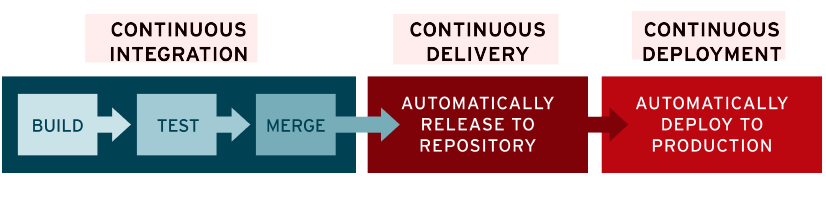
\includegraphics[scale=0.6]{media/CICD.png}  
   
\newpage

 \item \subsection*{Continuous Deployment Patterns}
   \addcontentsline{toc}{subsection}{Continuous Deployment Patterns}
	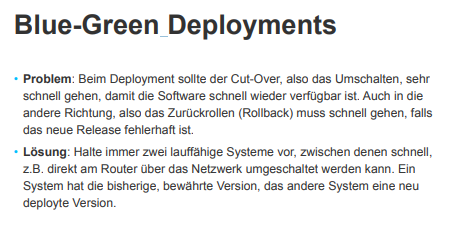
\includegraphics[scale=1.3]{media/blueGreenDep.png}\\
	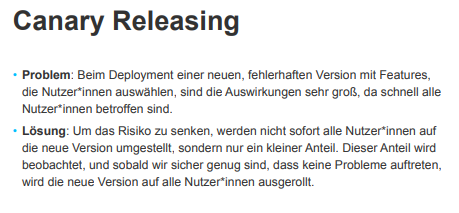
\includegraphics[scale=1.3]{media/canaryReleasing.png}\\
	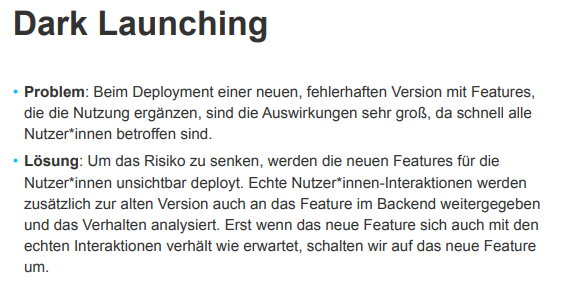
\includegraphics[scale=1.1]{media/darkLaunching.png}\\
	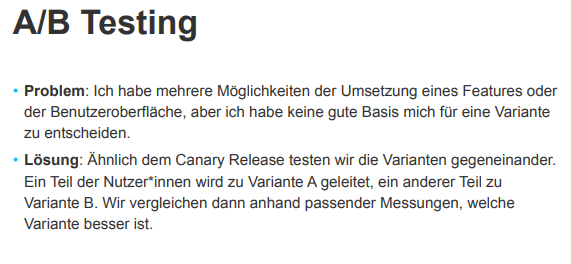
\includegraphics[scale=1.1]{media/A_B-Tests.png}\\
	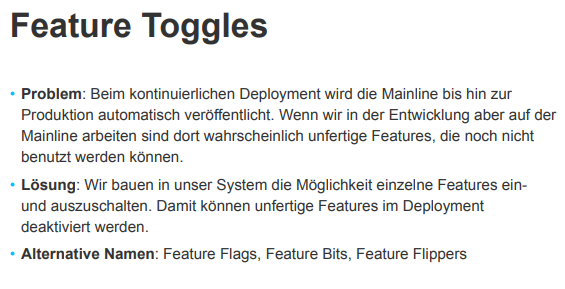
\includegraphics[scale=1.1]{media/featureToggles.png}
 
   \item \subsection*{Kontrollflussgraphen}
   \addcontentsline{toc}{subsection}{Kontrollflussgraphen}
   Ein Kontrollflussgraph ist eine grafische Darstellung, die zeigt, wie die Ausführung von Programmanweisungen oder Codeblöcken miteinander verbunden ist. Er hilft dabei, den Ablauf eines Programms zu visualisieren und die möglichen Ausführungspfade zu verstehen.\\
   
   \item \subsection*{Prüfresultate beim Testen}
   \addcontentsline{toc}{subsection}{Prüfresultate beim Testen}
   Ein \textbf{richtig positiver} Fehler tritt auf, wenn ein Test tatsächlich einen Fehler findet, der auch tatsächlich existiert.\\
   Ein \textbf{falsch positiver} Fehler tritt auf, wenn ein Test einen Fehler meldet, obwohl in Wirklichkeit kein Fehler vorhanden ist.\\
   Ein \textbf{richtig negativer} Fehler tritt auf, wenn ein Test keinen Fehler findet, und es gibt tatsächlich keinen Fehler.\\
   Ein \textbf{falsch negativer} Fehler tritt auf, wenn ein Test keinen Fehler findet, obwohl ein Fehler tatsächlich vorhanden ist.
   
   \item \subsection*{McCabes zyklomatische Komplexität}
   \addcontentsline{toc}{subsection}{McCabes zyklomatische Komplexität}
   Die zyklomatische Komplexität misst die Anzahl der linearen, unabhängigen Pfade durch den Programmcode. Diese Pfade entsprechen den möglichen Ausführungspfaden, die durch Verzweigungen (wie if-Bedingungen oder Schleifen) entstehen.
   
   \[
V(G) = E - N + 2
\]
wobei 
E die Anzahl der Kanten und 
N die Anzahl der Knoten im Kontrollflussgraphen ist.

	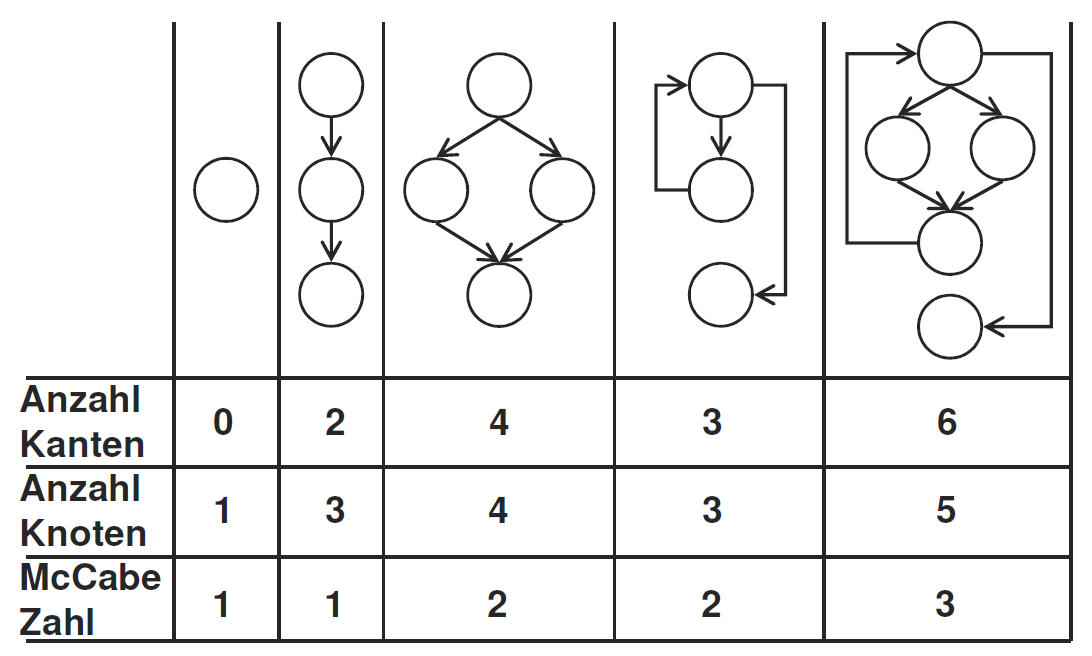
\includegraphics[scale=0.3]{media/McCabe.png}\\
	
\end{enumerate}
\newpage
\addcontentsline{toc}{section}{Projekt- und Produktmanagement}
\section*{Projekt- und Produktmanagement}
  \begin{enumerate}[label=\alph*)]
  
\addcontentsline{toc}{subsection}{Vorgehensmodelle}
  \subsection*{Vorgehensmodelle}
  
\addcontentsline{toc}{subsubsection}{Wasserfallmodell}
  \item \textbf{Wasserfallmodell}\\
  Im Wasserfallmodell „fließt“ eine Projektphase in die Nächste – immer in eine Richtung, ohne die Reihenfolge zu verändern, wie ein Wasserfall eben. Diese Methode ist das Gegenstück zum agilen Projektmanagement, bei dem Abläufe flexibel gestaltet und nicht direkt von Beginn an bis ins Detail definiert sind. Jede Phase im Wasserfallmodell baut auf der vorherigen auf und muss vollständig abgeschlossen sein, bevor die nächste Phase beginnen kann.\\
  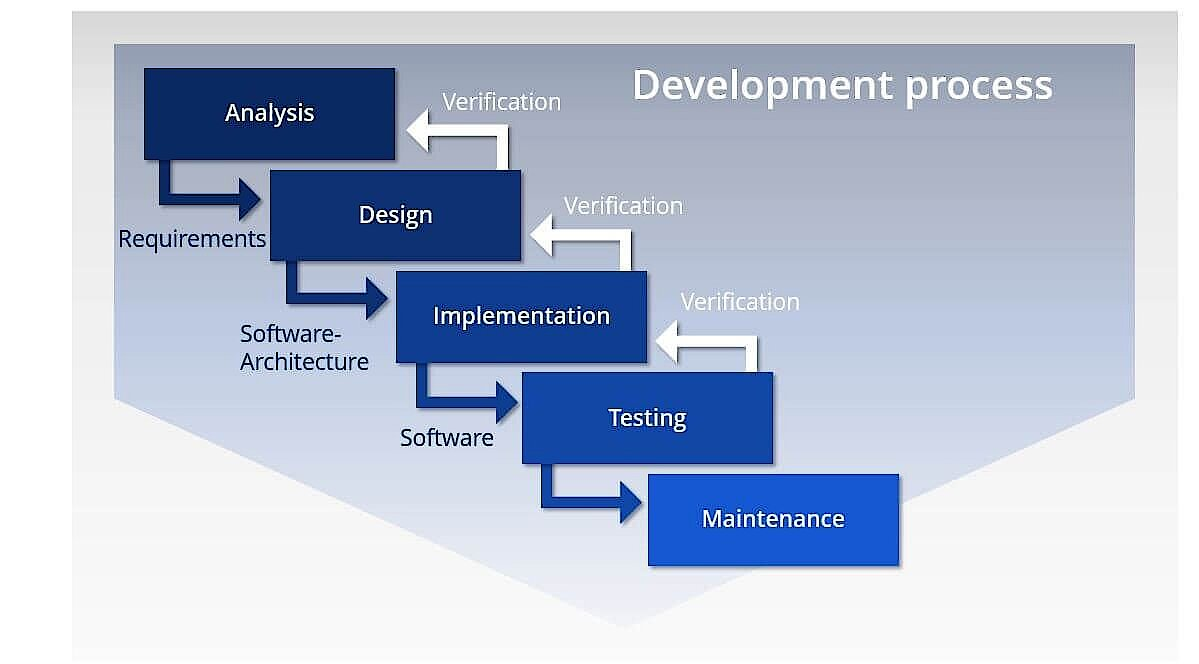
\includegraphics[scale=0.2]{media/Wasserfall.jpg}
  
\addcontentsline{toc}{subsubsection}{iterative Entwicklung}
  \item  \textbf{iterative Entwicklung}\\
  Das Prinzip der iterativen Entwicklung beruht darauf, dass ein Produkt durch permanente Wiederholungen (Iterationen) optimiert und zur Anwendungsfähigkeit gebracht wird.
In das Endprodukt gehen also alle Erfahrungen aus dem ersten Durchgang ein und auch neuere
Entwicklungen.
In jeder Iteration werden die Tätigkeiten Analysieren, Entwerfen, Codieren und Testen ausgeführt, und das
resultierende System wird erprobt.
Nach jeder Iteration sollte eine Abnahme mit dem Kunden erfolgen und so die Anforderungen und die Qualität der Software überprüft werden.\\
	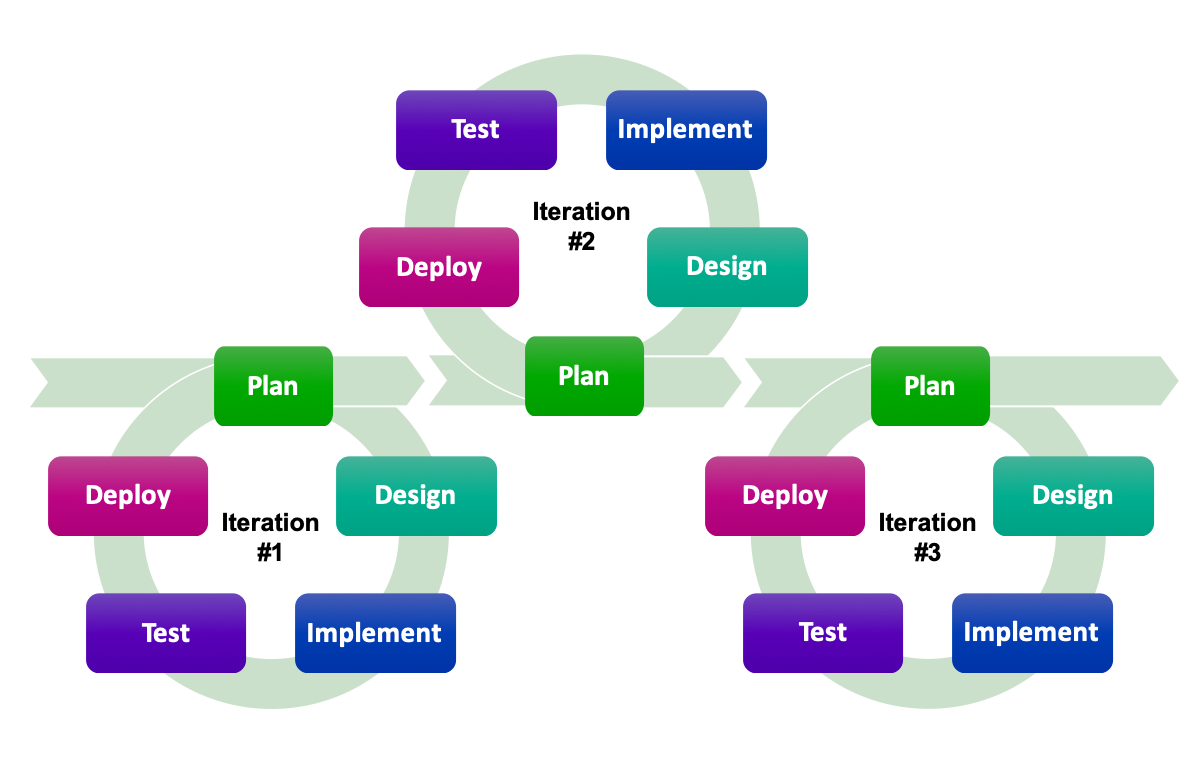
\includegraphics[scale=0.4]{media/iterativeEntwicklung.png}


  \item  \textbf{inkrementelle Entwicklung}\\
  \addcontentsline{toc}{subsubsection}{inkrementelle Entwicklung}
  Inkrementelle Entwicklung ist ein Softwareentwicklungsansatz, bei dem die Software schrittweise erstellt wird. Jede Entwicklungsphase liefert ein vollständiges und funktionsfähiges Produktinkrement, das auf den vorherigen Inkrementen aufbaut und zusätzliche Funktionen bietet.\\
  Ein Beispiel für den \textbf{Unterschied zwischen iterativ und inkrementell:}\\
Stellen wir uns vor, eine Dating-Website zu erstellen. Bei einer iterativen Arbeitsweise würde das Team ein wenig an jedem Teil der Seite arbeiten – Profilverwaltung, Suchfunktion, Werbeanzeigen etc. Danach kommt das Team dann auf alle einzelnen Teile zurück und verbessert diese.\\
Bei dieser rein iterativen Arbeitsweise wird also die gesamte Seite verbessert.\\

Wenn diese Website inkrementell erstellt würde, würde das Team beispielsweise erst die Profilverwaltung perfektionieren, bevor es die Suchfunktion fertiggestellt usw. Es wird also immer erst die gesamte Arbeit für einen Bereich abgeschlossen, ehe mit etwas Neuem begonnen wird.
	

	\item \subsubsection*{Scrum}
	\addcontentsline{toc}{subsubsection}{Scrum}
	Scrum ist ein Vorgehensmodell/Rahmenwerk zur agilen Softwareenticklung für die Zusammenarbeit von Teams basierend auf einer Definition von Rollen, Meetings und Werkzeugen, die einem Teamstruktur und einen klar definierten Arbeitsprozess basierend auf agilen Prinzipien geben.
	
	\begin{table}[ht]
	\begin{tabular}{|c|c|c|}
 	\hline
	 Rollen/Scrum Team & Ereignisse & Artefakte \\
	 \hline
 	 •Produktowner & •Der Sprint & •Product Backlog\\
 	 •Scrum Master & •Sprint-Planung & •Sprint Backlog\\
 	 •Developers & •Sprint- Review & •Inkrement\\
 	 & •Sprint- Retrospektive & \\
 	 & •Tägliches Scrum-Meeting &\\
	 \hline
\end{tabular}
\end{table}
    Ein Kunde hat einen Wunsch und geht zum \textbf{Product Owner} des Scrum-Teams. Zum Produktwunsch des Kunden gibt es meist eine Vision, die langfristig angibt, wohin sich das Produkt entwickeln soll. Aus dieser Vision, dem Produktziel und den Wünschen des Kunden erstellt und pflegt der Product Owner das \textbf{Product Backlog}. Es ist eine Liste von allen bekannten Anforderungen und zum aktuellen Zeitpunkt. Das Product Backlog ist mit Wünschen und Aufgaben gefüllt, die man \textbf{Product Backlog Items} nennt. Diese können im Format der User-Story gefüllt sein. Das Product Backlog besteht aus \textbf{Product Goal} (Ziel), welches das Commitment zum Product Backlog ist.

\textbf{Sprint Planning:} Diese besteht aus 3 Themen: Warum?, Was? und Wie?

Das \textbf{Sprint Backlog} ist immer eine Teilmenge vom Product Backlog. Während des Sprint Planning Meetings wählt das Scrum-Team dann eine Teilmenge der Items aus dem Product Backlog aus, die sie im kommenden Sprint bearbeiten möchten. Das Ergebnis des Sprint-Planning ist das Sprint Backlog und das dazugehörige Sprint Goal. 

Während des Sprints arbeiten alle Entwickler (oft im Pair-Programming) zusammen an Lösungen. Jeden Tag zur gleichen Zeit findet das \textbf{Daily Scrum} statt. Dort fragen sich die Entwickler, wie der Fortschritt auf dem Weg zum Sprint Goal ist. Dabei beantwortet jeder 3 Fragen:

- Was habe ich gestern gemacht?\\
- Was werde ich heute für das Sprintziel tun?\\
- Welche Probleme oder Hindernisse gibt es?\\

Irgendwann nach einer Zeit läuft die Zeitscheibe des Sprints ab und wir erzeugen ein \textbf{Increment}, was die fertige nutzbare Arbeit des Sprint darstellt. Damit die Qualität eingehalten wird, gibt es die \textbf{Definition of Done}, die sagt wann Arbeit als fertig gilt. Im \textbf{Sprint-Review} laden wir User, Stakeholder und Kunden ein und lassen uns über das Inkrement Feedback geben. Das Feedback fließt wieder in das Product Backlog ein. Während wir im Review auf das Produkt schauen, legen wir den Wert in der \textbf{Retrospektive} auf den Prozess. Wie hat die Zusammenarbeit geklappt? Verbesserungen gelangen wieder in das Sprint Backlog.

Der \textbf{Scrum Master} achtet hierbei auf das ganze Scrum- Konstrukt und die Sprints. Er ist verantwortlich für die Einhaltung von Scrumwerten und -techniken und repräsentiert das Management. Die typische Sprintdauer beträgt 2-4 Wochen.
  \end{enumerate}
  
  \newpage
  \subsection*{Organisationsformen für Teams}
\addcontentsline{toc}{subsection}{Organisationsformen für Teams}
	
	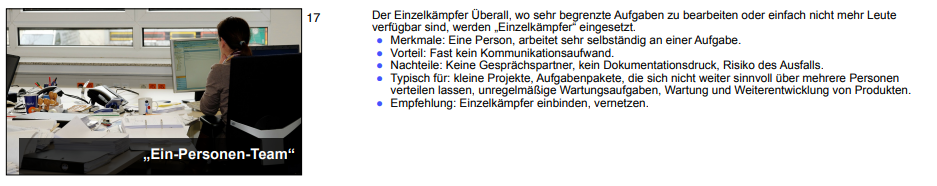
\includegraphics[scale=1.1]{media/Organisationsformen0.png}
	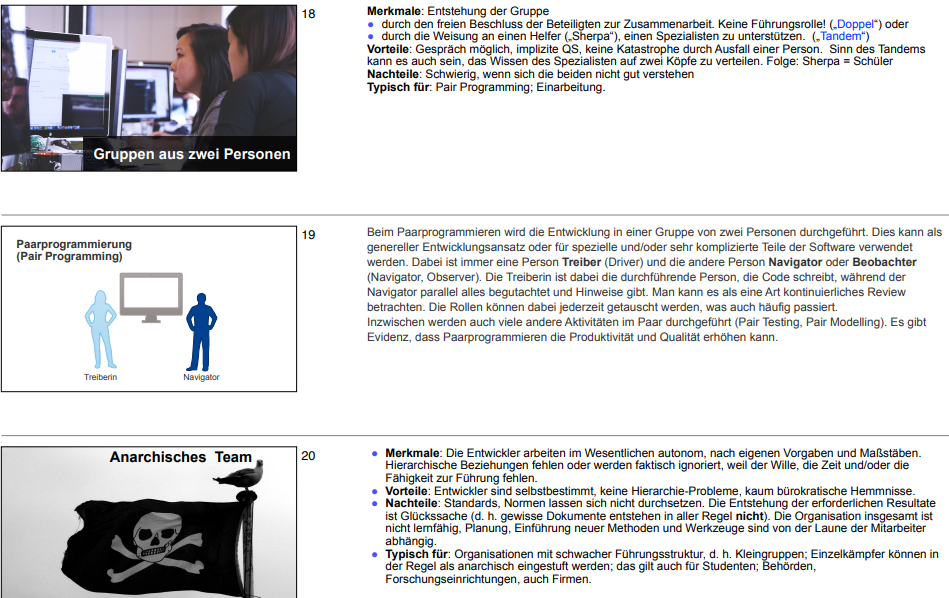
\includegraphics[scale=1.1]{media/Organisationsformen1.png}
	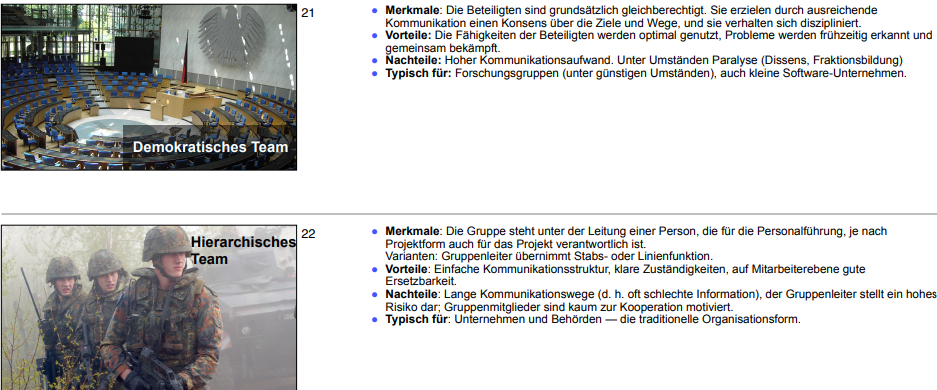
\includegraphics[scale=1.1]{media/Organisationsformen2.png}
	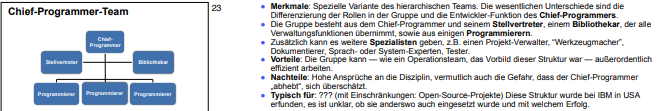
\includegraphics[scale=1.5]{media/Organisationsformen3.png}
	
  \subsection*{Unternehmensorganisation}
\addcontentsline{toc}{subsection}{Unternehmensorganisation}
	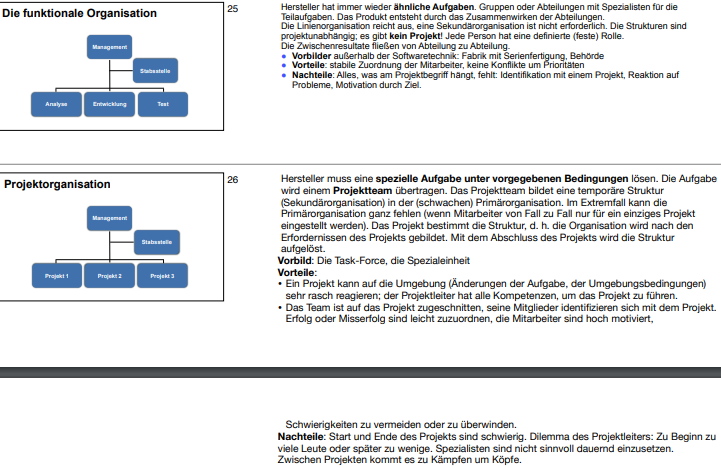
\includegraphics[scale=1.3]{media/Organisationsformen4.png}\\
	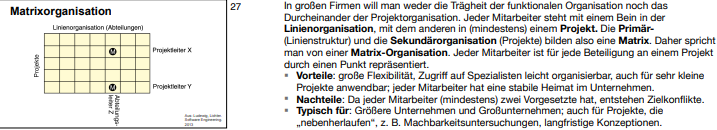
\includegraphics[scale=1.3]{media/Organisationsformen5.png}\\

	
	


\section*{Begriffe im Software Engineering}
\addcontentsline{toc}{section}{Begriffe im Software Engineering}
\subsection*{Prinzipien}
\addcontentsline{toc}{subsection}{Prinzipien}
\begin{enumerate}[label=\alph*)]
\item \textbf{Rationalität: }Ingenieur*innen sind Feinde des Aberglaubens, Verehrer der Zahlen und Formeln, also Kinder der Aufklärung
\item \textbf{Problemlösen: }Scientists build to learn, engineers learn to build
\item \textbf{Kostenbewusstsein statt Perfektionismus }
\item \textbf{Universeller Anspruch, der nicht vor Fachgrenzen Halt macht: }Ingenieur*innen kapitulieren nicht, wenn das Problem die Grenzen ihres Fachs überschreitet.
\item \textbf{Qualitätsbewusstsein als Denkprinzip }
\item \textbf{Die Einführung und Beachtung von Normen }
\item \textbf{Denken in Baugruppen }
\end{enumerate}

\subsection*{Weshalb sind beim „Progamming in the Large“ grundsätzlich andere
Techniken notig sind als beim „Programming in the Small“?}
\addcontentsline{toc}{subsection}{„Progamming in the Large“ vs. „Programming in the Small“}
Beim „Programming in the Large“ sind andere Techniken nötig, weil die Komplexität und der Umfang größer sind, was eine sorgfältige Planung der Architektur und umfassende Dokumentation erfordert. Zudem arbeiten hier oft mehrere Entwickler zusammen, was Koordination und Kommunikation mittels spezieller Werkzeuge und Methoden notwendig macht. Im Gegensatz dazu ist „Programming in the Small“ einfacher strukturiert, oft von Einzelpersonen durchgeführt, und benötigt weniger formale Prozesse.

\subsection*{Was ist der Unterschied zwischen Safety und Security?}
\addcontentsline{toc}{subsection}{Safety vs. Security}

Safety (Sicherheit im Sinne von Betriebssicherheit/ technische Sicherheit): Bezieht sich auf die Gewährleistung, dass ein System auch unter ungewöhnlichen oder fehlerhaften Bedingungen sicher funktioniert und keine Schäden verursacht. Es geht darum, Unfälle, Fehlfunktionen und Ausfälle zu verhindern, die zu physischen oder materiellen Schäden führen könnten.\\
Security (Sicherheit im Sinne von IT-Sicherheit/ Informationssicherheit): Bezieht sich auf den Schutz eines Systems vor böswilligen Angriffen, unbefugtem Zugriff und Datenverlust. Es geht darum, die Vertraulichkeit, Integrität und Verfügbarkeit von Daten und Diensten zu gewährleisten.\\

\underline{Beispiel für eine Software, bei der Security eine wichtige Anforderung ist, nicht jedoch Safety:}\\
Online-Banking-Anwendung: Hier ist Security besonders wichtig, um die finanziellen Daten der Benutzer vor unbefugtem Zugriff und Betrug zu schützen. Safety ist weniger relevant, da keine physischen oder materiellen Schäden drohen.\\
\underline{Beispiel für eine Software, bei der Safety in besonderem Maß wichtig ist:}\\
Medizinische Geräte-Software (z.B. für Herzschrittmacher): Hier ist Safety besonders wichtig, da Fehlfunktionen oder Ausfälle direkt zu lebensbedrohlichen Situationen für die Patienten führen können. Security ist ebenfalls wichtig, aber die unmittelbare Betriebssicherheit hat oberste Priorität.
\subsection*{Stakeholder (Interessenten an der Entwicklung und dem Betrieb)}
\addcontentsline{toc}{subsection}{Stakeholder im Software Engineering}
Stakeholder sind Personen oder Gruppen, die ein Interesse oder einen Einfluss auf ein Projekt haben.\\
\textbf{Endbenutzer:} Personen, die die Software täglich nutzen und deren Anforderungen erfüllt werden müssen.\\
\textbf{Kunden/Klienten:} Auftraggeber der Software, die sicherstellen möchten, dass das Produkt ihren Bedürfnissen entspricht.\\
\textbf{Projektmanager:} Verantwortlich für die Planung, Durchführung und Überwachung des Projekts, um sicherzustellen, dass es termingerecht und im Budget bleibt.\\
\textbf{Projektleiter:} Verantwortlich für die Gesamtplanung, Durchführung und Überwachung des Projekts. Sorgt dafür, dass das Projekt termingerecht, im Budget und entsprechend den Anforderungen abgeschlossen wird. Koordiniert Kommunikation zwischen den Stakeholdern und löst auftretende Probleme.\\
\textbf{Entwicklungsteam:} Entwickler, die für das Design, die Implementierung und das Testen der Software verantwortlich sind.\\
\textbf{QA-Team:} Qualitätssicherungsmitarbeiter, die Tests durchführen, um sicherzustellen, dass die Software den Qualitätsstandards entspricht.\\

\subsection*{Qualitätenbaum}
\addcontentsline{toc}{subsection}{Qualitätenbaum}
\includegraphics[scale=0.52]{media/Qualitätenbaum.png}

\subsection*{Die QS-Ingenieur*in}
\addcontentsline{toc}{subsection}{Die QS-Ingenieur*in}
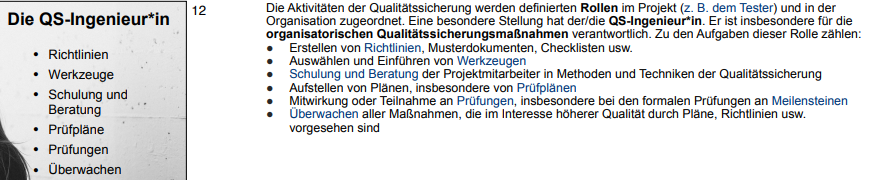
\includegraphics[scale=1.18]{media/QS_Ingenieur.png}

\subsection*{Software-Review}
\addcontentsline{toc}{subsection}{Software-Review}

Eine Software-Review ist eine formelle oder informelle Methode zur Bewertung der Qualität, des Designs und der Funktionalität von Software durch eine oder mehrere Personen, die nicht direkt an der Entwicklung der überprüften Software beteiligt sind. Ziel ist es, Fehler und Schwächen frühzeitig zu identifizieren, die Qualität zu verbessern und sicherzustellen, dass die Software den festgelegten Anforderungen und Standards entspricht.
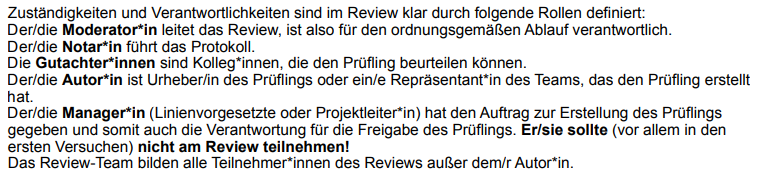
\includegraphics[scale=1.18]{media/Review.png}\\
\textbf{Nachteile von Tests im Vergleich zu Review z.bsp.}\\
Aussagekraft des Tests wird überschätzt, zeigt nicht Korrektheit, denn schon die Zustandsräume kleiner Programme sind riesig, Man kann nicht alle Anwendungssituationen nachbilden, Der Test zeigt nur die Existenz von Fehlern und nicht die Fehlerursache oder dass keine vorhanden sind.\\
Testabdeckung misst nur den Teil des Codes der ausgeführt wird, aber nicht wie gründlich sie sind.
\section*{Prüfungsfragen}
\addcontentsline{toc}{section}{Prüfungsfragen}
\addcontentsline{toc}{subsection}{1. Aspekte, die ein Entwurf gegenüber den Anforderungen zusätzlich enthalten sollte.}
\textbf{1. Aspekte, die ein Entwurf gegenüber den Anforderungen zusätzlich enthalten sollte:}\\
\underline{Anforderungen:} Fokus auf \textbf{was} das System tun soll.\\
\underline{Entwurf:} Fokus auf \textbf{wie} das System die Anforderungen technisch umsetzen wird.\\
Was ist im Entwurf, aber nicht in den Anforderungen?: Diagramme, Art der Datenspeicherung, Architektur (Struktur), Aufteilung der Komponenten, verwendete Programmiersprache, APIs \\
\addcontentsline{toc}{subsection}{2. Software ist inmateriell. Erkläre}
\textbf{2. Software ist inmateriell. Erkläre}\\
Software ist kein physisches Objekt, das man anfassen oder sehen kann. Stattdessen besteht Software aus digitalen Daten, die auf einem Computer oder einem anderen digitalen Gerät gespeichert sind. Sie läuft also auf physischen Geräten und man kann mit ihr interagieren. Die immaterielle Natur von Software hat weitreichende Auswirkungen auf ihre Entwicklung, Verteilung, Nutzung und rechtliche Behandlung.\\
\addcontentsline{toc}{subsection}{3. Prozessqualität vs. Produktqualität}
\textbf{3. Prozessqualität vs. Produktqualität}\\
Während Prozessqualität darauf abzielt, die Effizienz, Konsistenz und Verbesserung der Abläufe zu maximieren, indem zB Fehler vermieden und behandelt werden, konzentriert sich Produktqualität auf die Eigenschaften und die Zufriedenheit der Endnutzer des Produkts, also die Zuverlässigkeit, Benutzerfreundlichkeit, Funktionalität und Haltbarkeit. Beide Aspekte sind eng miteinander verbunden, da eine hohe Prozessqualität oft zu einer besseren Produktqualität führt. Ein gut strukturierter und effizienter Prozess kann die Wahrscheinlichkeit von Fehlern reduzieren und die Produktion von qualitativ hochwertigen Produkten sicherstellen.\\
\addcontentsline{toc}{subsection}{4. 2 Analysetechniken, die sich besonders gut zur Feststellung des Ist-Zustandes eignen}
\textbf{4. 2 Analysetechniken, die sich besonders gut zur Feststellung des Ist-Zustandes eignen}\\
Die \underline{SWOT-Analyse} bietet eine umfassende Bewertung der internen und externen Faktoren, die den aktuellen Zustand beeinflussen.\\
- Bietet eine strukturierte und umfassende Analyse.\\
- Einfach anzuwenden und zu verstehen. \\
- Hilft, sowohl interne als auch externe Faktoren zu berücksichtigen.\\
\underline{Prozessanalyse} ermöglicht eine detaillierte Untersuchung der bestehenden Abläufe. \\
- Detaillierte und klare Visualisierung der aktuellen Abläufe.\\
- Ermöglicht die Identifikation spezifischer Probleme und Verbesserungsmöglichkeiten.\\
- Grundlage für die Prozessoptimierung und Neugestaltung.\\
\addcontentsline{toc}{subsection}{5. Was ist Software Alterung?}
\textbf{5. Was ist Software Alterung?}\\
Software-Alterung beschreibt den Prozess, bei dem Software im Laufe der Zeit an Leistungsfähigkeit und Zuverlässigkeit verliert, auch wenn sie nicht aktiv genutzt wird. Dieser Effekt kann durch verschiedene Faktoren verursacht werden, die sowohl auf der Software selbst als auch auf ihrer Umgebung basieren. \\
Ursachen: Ressourcenlecks, Datenkorruption, Software- und Systemänderungen, Änderungen in der Nutzung\\
Symptome: Leistungsabfall, Erhöhte Fehlerraten, Ressourcenerschöpfung, Unerwartetes Verhalten\\
\addcontentsline{toc}{subsection}{6. Nenne ein Dokumententyp, der nicht geeignet ist durch ein Review geprüft zu werden}
\textbf{6. Nenne ein Dokumententyp ,der nicht geeignet ist durch ein Review geprüft zu werden}\\
Ein Dokumententyp, der nicht geeignet ist durch ein Review bzw. durch einen Test geprüft zu werden, sind persönliche Notizen.\\
Warum nicht für Reviews geeignet? Subjektiver Inhalt, Nicht für die Öffentlichkeit bestimmt, Mangel an formaler Struktur\\
Warum nicht für Tests geeignet? Kein formalisierter Inhalt, Fehlende Zielsetzungen, Unstrukturierte Informationen\\
\addcontentsline{toc}{subsection}{7. Erkläre die Make or Buy-Entscheidung und Argumente für und gegen die Neuentwicklung}
\textbf{7. Erkläre die Make or Buy-Entscheidung und Argumente für und gegen die Neuentwicklung}\\
Die Make-or-Buy-Entscheidung im Software Engineering bezieht sich auf die strategische Entscheidung, ob eine Softwarelösung intern entwickelt (Make) oder extern beschafft (Buy) werden soll. Diese Entscheidung basiert auf einer Vielzahl von Faktoren, darunter Kosten, Zeit, Ressourcen und strategische Ziele des Unternehmens.\\
- für die Neuentwicklung:  Eine intern entwickelte Software kann exakt auf die spezifischen Bedürfnisse und Anforderungen des Unternehmens zugeschnitten werden. Dies ermöglicht eine höhere Anpassungsfähigkeit und Flexibilität, um spezifische Geschäftsprozesse und -anforderungen zu erfüllen. \\
- gegen die Neuentwicklung: Die Entwicklung einer maßgeschneiderten Softwarelösung kann sehr kostspielig und zeitaufwendig sein. Dies umfasst nicht nur die initialen Entwicklungs- und Implementierungskosten, sondern auch die langfristigen Wartungs- und Updatekosten.
\newpage
\addcontentsline{toc}{subsection}{8. Fehlhandlung(Mistake) und Ausfall(Failure)/ Fehlerursache(Fault) und Fehlerzustand(Error)}
\textbf{8. Fehlhandlung(Mistake) und Ausfall(Failure)/ Fehlerursache(Fault) und Fehlerzustand(Error)}\\
- Fehlhandlung(Mistake): Eine Fehlhandlung ist eine menschliche Aktion, die zu einem Fehler führt. Dies kann durch Unachtsamkeit, Missverständnisse oder mangelndes Wissen geschehen, kann aber auch durch andere menschliche Fehler verursacht werden, wie z.B. bei der Anforderungsanalyse, beim Design oder bei der Dokumentation.\\
- Fehlerursache(Fault,Bug): Eine Fehlerursache ist die zugrundeliegende Ursache für einen Fehlerzustand. Es ist der eigentliche Defekt im System, der durch eine Fehlhandlung eingebracht wurde.Die Stelle, die falsch implementiert ist, ist dann die Fehlerursache.\\
- Fehlzustand(Error): Ein Fehlerzustand ist der Zustand eines Systems, der von der Spezifikation abweicht, verursacht durch eine Fehlhandlung, aber noch nicht notwendigerweise ein Ausfall passiert ist. Ein Fehlerzustand repräsentiert eine interne Abweichung des Systems.\\
- Ausfall(Failure):  Ein Ausfall tritt auf, wenn ein System sein vorgesehenes Verhalten nicht erfüllt, also wenn ein Fehlerzustand nach außen sichtbar wird und die Funktionalität des Systems beeinträchtigt. Ein Ausfall kann sich auf verschiedene Arten äußern, z.B. als Absturz, als falsche Berechnung, als unvollständige Ausgabe oder als unerwartetes Verhalten. Der Benutzer bemerkt, dass das System nicht (mehr) den geforderten Dienst erbringt.
- Defekt (Defect): Generische Bezeichnung für Ausfall und Fehlerursache\\
\addcontentsline{toc}{subsection}{9. Alles zu Risikomanagement}
\textbf{9. Alles zu Risikomanagement}\\
Das Ziel des Risikomanagements in der Softwareentwicklung ist es, potenzielle Risiken frühzeitig zu identifizieren, zu bewerten und geeignete Maßnahmen zu ergreifen, um die negativen Auswirkungen dieser Risiken auf das Projekt und das Endprodukt zu minimieren oder zu verhindern. Dadurch sollen die Wahrscheinlichkeit und die Folgen unerwünschter Ereignisse reduziert werden, um die Projektziele zu erreichen und die Qualität der Software zu gewährleisten.\\
Warum ist Risikomanagement wichtig? Vermeidung von Projektverzögerungen, Kosteneffizienz, Qualitätssicherung, Stakeholder-Vertrauen, Kontinuierliche Verbesserung\\
\underline{Top 10 Risk Items} \\
1. Personelle Probleme \\
2. Unrealistische Zeit- und Kostenpläne \\
3. Entwicklung der falschen Funktionalität \\
4. Entwicklung der falschen Benutzeroberfläche \\
5. Gold Plating \\
6. Kontinuierlicher Strom von Anforderungsänderungen \\
7. Probleme mit extern durchgeführter Aufgaben \\
8. Probleme mit extern entwickelten Komponenten \\
9. Probleme mit Echtzeit-Performanz \\
10. Überforderung der Möglichkeiten der Informatik \\
\underline{Gegenmaßnahmen:} \\
1. Top-Talente als Mitarbeiter, passende Profile, Team-Building, Morale-Building, Cross-Training, Schlüsselpersonen früh ins Projekt \\
2. Detaillierte Kosten- und Zeitplanung basierend auf verschiedenen Quellen, Design to Cost, inkrementelle Entwicklung, Wiederverwendung, Anforderungen zurückstellen \\
3. Organisationsanalyse, Nutzungsanalyse, Formulierung eines Einsatzkonzepts, Nutzerbefragung, Prototyping, frühes Benutzerhandbuch \\
4. Prototyping, Szenarien, Nutzungssanalyse \\
5. Anforderungen zurückstellen, Prototyping, Kosten/Nutzen-Analyse, Design to Cost \\
6. Hohe Änderungsschwelle, inkrementelle Entwicklung \\
7. Referenzen prüfen, Team Building, Prüfungen vor der Auftragsvergabe, Prototyping, Beauftragung mehrerer Zulieferer \\
8. Benchmarking, Inspektionen, Referenzen prüfen, Kompatibilitätsanalyse \\
9. Simulation, Benchmarking, Modellierung, Prototyping, Instrumentierung, Tuning \\
10.Technische Analyse, Kosten/Nutzen-Analyse, Prototyping \\
\addcontentsline{toc}{subsection}{10. Was ist ein Arbeitspaket, woraus besteht es (durch welche Informationen ist es definiert)?}
\textbf{10. Was ist ein Arbeitspaket, woraus besteht es (durch welche Informationen ist es definiert)?}\\
Ein Arbeitspaket repräsentiert eine spezifische Aufgabe oder eine Gruppe von Aufgaben, die durchgeführt werden müssen, um ein Projektziel zu erreichen. Arbeitspakete sind dabei so klein und spezifisch, dass sie klar definiert und handhabbar sind. In der Software-Entwicklung bestehen Arbeitspakete typischerweise aus folgenden Elementen:\\
Titel/Bezeichnung, Beschreibung, Ziele und Akzeptanzkriterien, Verantwortlichkeiten/Rollen, Zeitplan, Abhängigkeiten, Ressourcen, Ergebnisse/Deliverables, Risiken und Annahmen, Aufwandschätzung \\
Ein Arbeitspaket hilft dabei, ein Projekt in überschaubare Teile zu zerlegen, die effektiv geplant, überwacht und kontrolliert werden können. Es fördert die klare Kommunikation und Verantwortlichkeit innerhalb des Teams und stellt sicher, dass alle Beteiligten ein gemeinsames Verständnis der Aufgaben und Ziele haben.\\
\addcontentsline{toc}{subsection}{11. Nenne 3 Beispiele für nichtfunktionale Anforderungen}
\textbf{11. Nenne 3 Beispiele für nichtfunktionale Anforderungen}\\
- \underline{Performance:} Das System muss in der Lage sein, mindestens 1000 Transaktionen pro Sekunde zu verarbeiten. Antwortzeiten für Benutzeranfragen dürfen nicht länger als 2 Sekunden betragen.\\
- \underline{Sicherheit:} Alle Datenübertragungen müssen durch SSL/TLS verschlüsselt werden. Benutzer müssen sich über ein zweistufiges Authentifizierungsverfahren anmelden.\\
- \underline{Zuverlässigkeit/Verfügbarkeit:} Das System muss eine Verfügbarkeit von 99,9\% während der Geschäftszeiten garantieren. Im Falle eines Systemausfalls muss das System innerhalb von 1 Stunde wiederhergestellt werden können.\\
\addcontentsline{toc}{subsection}{12. Aufwandsschätzung}
\textbf{12. Aufwandsschätzung}\\
Wie viel Zeit wird benötigt, um das Arbeitspaket oder das gesamte Projekt abzuschließen?
Welche Ressourcen werden benötigt, um die Aufgaben erfolgreich zu erledigen?\\
Warum brauchen wir in der Softwareplanung eine Aufwandschätzung?\\
- Projektplanung und -kontrolle:
Eine präzise Aufwandsschätzung ermöglicht eine realistische Projektplanung. Sie hilft dabei, den zeitlichen Rahmen und die benötigten Ressourcen zu bestimmen, was wiederum die Erstellung eines detaillierten Projektplans erleichtert. Ohne eine solche Schätzung besteht die Gefahr, dass Projekte zu lange dauern oder die verfügbaren Ressourcen überschreiten.\\
- Budgetierung und Ressourcenmanagement:
Aufwandschätzungen sind entscheidend für die Budgetplanung. Sie ermöglichen es, die Kosten für ein Projekt im Voraus zu berechnen und sicherzustellen, dass ausreichend finanzielle und personelle Ressourcen zur Verfügung stehen. Dies hilft, finanzielle Überziehungen zu vermeiden und sicherzustellen, dass die richtigen Fähigkeiten und Kapazitäten zur Verfügung stehen, um das Projekt erfolgreich abzuschließen.\\
\addcontentsline{toc}{subsection}{13. Beschreiben Sie, was Planning Poker ist.}
\textbf{13. Beschreiben Sie, was Planning Poker ist.}\\
Planning Poker ist eine agile Methode zur Schätzung des Aufwands in Softwareentwicklungsprojekten, die oft in Scrum-Teams verwendet wird. Es ist eine kollaborative Technik, bei der das gesamte Team beteiligt ist, um den Arbeitsaufwand für User Stories oder andere Arbeitspakete zu schätzen. Der Prozess fördert die Diskussion und den Austausch von Wissen innerhalb des Teams und hilft, eine realistischere und konsensbasierte Schätzung zu erzielen. \\
\addcontentsline{toc}{subsection}{14. Fasse Protoyping zusammen.}
\textbf{14. Fasse Protoyping zusammen.}\\
Prototyping ist ein iterativer Entwicklungsansatz in der Software-Entwicklung, bei dem ein vorläufiges Modell oder eine frühe Version eines Produkts erstellt wird, um verschiedene Aspekte des Endprodukts zu testen und zu validieren. Ziel des Prototyping ist es, Feedback von Nutzern und Stakeholdern zu erhalten, um Anforderungen besser zu verstehen und das Design zu verfeinern, bevor das vollständige System entwickelt wird.\\
\addcontentsline{toc}{subsection}{15. Ebenen beim Entwurf (einer Software)}
\textbf{15. Ebenen beim Entwurf (einer Software)}\\
- Systemebene: Fokus auf das Gesamtsystem und seine Umgebung. \\
- Softwarearchitekturebene: Definiert die grundlegende Struktur und die Interaktionen der Hauptkomponenten der Software. \\
- Detailliertes Design: Spezifiziert das Design und die Implementierung einzelner Module und Komponenten. \\
- Implementierungsebene: Konkrete Programmierung und Codierung der Software. \\
Die Softwarearchitektur gehört zur Softwarearchitekturebene und bildet das Rückgrat des Softwareentwurfs, indem sie die Struktur, die Interaktionen und die grundlegenden Prinzipien festlegt, die die gesamte Softwareentwicklung leiten. Sie stellt sicher, dass das System den funktionalen und nicht-funktionalen Anforderungen entspricht und eine solide Basis für die weitere Detaillierung und Implementierung bietet.\\
\addcontentsline{toc}{subsection}{16. Durch was wird der Nutzen einer Software beeinflusst?}
\textbf{16. Durch was wird der Nutzen einer Software beeinflusst?}\\
Der Nutzen einer Software wird durch eine Vielzahl von Faktoren beeinflusst: Funktionalität, Benutzerfreundlichkeit, Zuverlässigkeit, Leistung, Sicherheit oder Wartbarkeit \\
\addcontentsline{toc}{subsection}{17. Use Cases vs. User Stories}
\textbf{17. Use Cases vs. User Stories}\\
Use Cases und User Stories sind beide Methoden zur Dokumentation und Definition von Anforderungen in der Softwareentwicklung, unterscheiden sich jedoch in ihrer Detaillierung und Herangehensweise.\\
- User Stories sind kurze, einfache Beschreibungen von Funktionen oder Anforderungen aus der Sicht eines Endbenutzers. Sie folgen typischerweise dem Format: Als [Rolle] möchte ich [Funktion], um [Ziel] zu erreichen.\\
- Use Cases sind detaillierte Beschreibungen der Interaktionen zwischen einem Benutzer (oder einem externen System) und der Software, um ein bestimmtes Ziel zu erreichen. Sie umfassen oft die Schritte, die durchgeführt werden müssen, um ein bestimmtes Ergebnis zu erzielen.\\
User Stories bieten eine schnelle, benutzerzentrierte Sicht auf die Anforderungen, während Use Cases detaillierte Szenarien und Abläufe liefern.
User Stories sind ideal für agile Umgebungen, in denen Flexibilität und schnelle Anpassungen wichtig sind. Use Cases sind besser geeignet, wenn ein detailliertes Verständnis der Systeminteraktionen erforderlich ist, z.B. in einer Phase der detaillierten Planung oder Analyse.\\
\addcontentsline{toc}{subsection}{18. Was ist die Rolle des Software Architekten?}
\textbf{18. Was ist die Rolle des Software Architekten?}\\
Die Rolle des Softwarearchitekten ist entscheidend für den Erfolg eines Softwareprojekts. Er oder sie ist verantwortlich für die Entwicklung und Dokumentation der Softwarearchitektur, die als Grundlage für die Implementierung und Wartung des Systems dient.\\
- Architekturentwurf \\
- Anforderungsanalyse \\
- Technologiewahl \\
- Sicherstellung der Qualitätsmerkmale \\
- Kommunikation und Dokumentation \\
- Unterstützung der Implementierung \\
- Qualitätskontrolle und Refactoring \\
- Risikomanagement \\
\addcontentsline{toc}{subsection}{19. Software-Krise und Ursachen}
\textbf{19. Software-Krise und Ursachen}\\
Die Software-Krise beschreibt eine Reihe von Herausforderungen und Problemen, die in den frühen Tagen der Softwareentwicklung auftraten, als die Industrie begann, zunehmend komplexe Softwareprojekte zu realisieren. Das Schlagwort Software-Krise entstand in den 1960er Jahren, als die Schwierigkeiten im Umgang mit der wachsenden Komplexität und dem Bedarf an zuverlässiger und wartbarer Software offensichtlich wurden.\\
Ursachen: \\
- Komplexität der Software
- Unzureichende Entwicklungsprozesse
- Mangelnde Planung und Dokumentation
- Fehlende Wartbarkeit und Zuverlässigkeit
- Unzureichende Testmethoden\\
\addcontentsline{toc}{subsection}{20. Der Begriff der Qualitätssicherung war in drei Teilbegriffe(Schwerpunkte) zerlegt worden. Welche?}
\textbf{20. Der Begriff der Qualitätssicherung war in drei Teilbegriffe(Schwerpunkte) zerlegt worden. Welche sind das?}\\
- Organisatorische Maßnahmen: Diese umfassen die Strukturierung und Planung des gesamten Softwareentwicklungsprozesses. Dazu gehören die Definition von Prozessen, Standards und Richtlinien, die Organisation von Teams und die Implementierung von Managementmethoden, um sicherzustellen, dass alle Aspekte der Softwareentwicklung effizient und zielgerichtet ablaufen.\\
- Konstruktive Maßnahmen: Hierbei geht es um die Schaffung einer soliden Basis für die Softwareentwicklung durch gute Design- und Entwicklungspraktiken. Dies umfasst unter anderem die Anwendung bewährter Methoden in der Softwarearchitektur, das Einhalten von Coding-Standards und das Nutzen von Entwurfsmustern, um eine hohe Qualität des entwickelten Codes zu gewährleisten.\\
- Analytische Maßnahmen: Diese beziehen sich auf die systematische Überprüfung und Bewertung der Software, um Fehler zu identifizieren und die Qualität zu sichern. Dazu gehören Software-Prüfungen wie Unit-Tests, Integrationstests, Systemtests und andere Testmethoden, die eingesetzt werden, um sicherzustellen, dass die Software die festgelegten Anforderungen erfüllt und funktionsfähig ist.\\
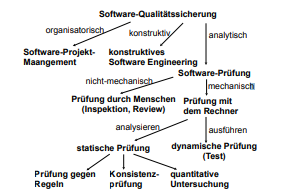
\includegraphics[scale=1.3]{media/QA.png}\\
\addcontentsline{toc}{subsection}{21. Welche Nachteile hat es, im Test Fehler zu beheben sobald sie aufgetreten sind?}
\textbf{21. Welche Nachteile hat es, im Test Fehler zu beheben sobald sie aufgetreten sind?}\\
Das Beheben von Fehlern erst während der Testphase kann zu erhöhten Kosten, Zeitverzögerungen, zusätzlicher Komplexität und reduzierter Testeffizienz führen. Es beeinträchtigt auch die Fähigkeit, die zugrunde liegenden Ursachen von Problemen zu identifizieren und zu adressieren. Idealerweise sollten Fehler so früh wie möglich im Entwicklungsprozess identifiziert und behoben werden, um diese Nachteile zu minimieren. Dies kann durch präventive Maßnahmen wie sorgfältige Anforderungsanalyse, Designüberprüfung, kontinuierliche Integration und frühzeitiges Testen erreicht werden.\\
\addcontentsline{toc}{subsection}{22. Welche Voraussetzungen müssen erfüllt sein damit mehrere Personen ein demokratisches Team bilden können?}
\textbf{22. Welche Voraussetzungen müssen erfüllt sein damit mehrere Personen ein demokratisches Team bilden können?}\\
Die Beteiligten sind grundsätzlich gleichberechtigt. Sie erzielen
durch ausreichende Kommunikation einen Konsens über die Ziele und Wege und sie verhalten sich diszipliniert. \\
- Klare Kommunikation und Transparenz \\
- Gegenseitiger Respekt und Vertrauen \\
- Gleichberechtigung \\
- Gemeinsame Ziele und Werte \\
- Teamarbeit\\
\addcontentsline{toc}{subsection}{23. Was versteht man unter einem quantifizierten Qualitätsmodell, und wie kann man es nutzen?}
\textbf{23. Was versteht man unter einem quantifizierten Qualitätsmodell, und wie kann man es nutzen?}\\
Ein quantifiziertes Qualitätsmodell ist ein System zur Bewertung und Messung der Qualität von Software oder anderen Produkten auf einer quantitativen Basis. Es definiert und verwendet Metriken und Kennzahlen, um die verschiedenen Aspekte der Qualität zu messen und zu bewerten. Diese Art von Modell ermöglicht eine objektive und messbare Beurteilung der Qualität, im Gegensatz zu subjektiven Bewertungen oder allgemeinen Beschreibungen.\\
Nutzen: \\
- Qualitätsbewertung \\
- Fehleridentifikation und -management \\
- Qualitätsverbesserung \\
- Vergleich und Benchmarking \\
- Kommunikation und Reporting \\
- Risikomanagement \\
\addcontentsline{toc}{subsection}{24. Warum sind Meilensteine in der Software-Entwicklung wichtig?}
\textbf{24. Warum sind Meilensteine in der Software-Entwicklung wichtig?}\\
Meilensteine sind essenziell für die erfolgreiche Durchführung von Softwareprojekten. Sie bieten Struktur, ermöglichen Fortschrittsüberwachung, erleichtern die Kommunikation und helfen bei der Steuerung und Risikomanagement. Durch die Definition und das Erreichen von Meilensteinen können Teams und Projektleiter sicherstellen, dass das Projekt zielgerichtet und effizient voranschreitet. \\
\addcontentsline{toc}{subsection}{25. Geben Sie zwei Gründe an, warum Anforderungen schriftlich festgehalten werden sollten.}
\textbf{25. Geben Sie zwei Gründe an, warum Anforderungen schriftlich festgehalten werden sollten.}\\
Das schriftliche Festhalten von Anforderungen ist entscheidend, um Klarheit und Verständlichkeit zu gewährleisten sowie um Nachvollziehbarkeit und Verfolgbarkeit sicherzustellen. Es hilft, Missverständnisse zu vermeiden, Änderungen zu dokumentieren und als rechtlich verbindliches Referenzdokument zu dienen\\
\addcontentsline{toc}{subsection}{26. Entwicklungs- und Evolutionsmodell für Mitarbeiter}
\textbf{26. Stellen Sie sich vor, es wurde eine neue Abteilung an der Uni für Software-Qualitätssicherung eingerichtet. Da die meisten Mitarbeiter der Meinung waren, dass Software-Evolution und Wartung weniger wichtig sind, haben sich die Mitarbeiter nicht mit Evolution und Wartung beschäftigt. Welches Entwicklungs- und Evolutionsmodell würden Sie für die Mitarbeiter der Abteilung für Software-Qualitätssicherung empfehlen?}\\
Die Abteilung für Software-Qualitätssicherung sollte ein agiles Entwicklungsmodell mit starkem Fokus auf Qualitätssicherung implementieren. Agile Methoden wie Scrum und Testgetriebene Entwicklung (TDD) ermöglichen iterative Entwicklung, kontinuierliche Verbesserung und enge Zusammenarbeit. Tools wie Continuous Integration/Continuous Delivery (CI/CD) und statische Codeanalyse unterstützen dabei, die Softwarequalität zu gewährleisten und schnelle Anpassungen an veränderte Anforderungen vorzunehmen. Durch regelmäßige Schulungen und einen Kulturwandel kann die Abteilung die Bedeutung von Software-Evolution und Wartung anerkennen und langfristig hochwertige, anpassungsfähige Software liefern.
\end{document}
